\documentclass[12pt,a4paper,oneside]{report}

% ── Encodage & Langue ─────────────────────────────────────────────────────────
\usepackage[utf8]{inputenc}
\usepackage[T1]{fontenc}
\usepackage[french]{babel}
\usepackage{textcomp}

% Déclarations Unicode de Robustesse
\DeclareUnicodeCharacter{00B0}{\textdegree}
\DeclareUnicodeCharacter{0153}{\oe}
\DeclareUnicodeCharacter{0152}{\OE}
\DeclareUnicodeCharacter{00A0}{~}
\DeclareUnicodeCharacter{202F}{\,}
\DeclareUnicodeCharacter{2019}{'}
\DeclareUnicodeCharacter{2018}{`}
\DeclareUnicodeCharacter{2014}{\textemdash}
\DeclareUnicodeCharacter{2013}{\textendash}

% ── Marges & Mise en Page (Standard TEK-UP : 2.5cm) ───────────────────────────
\usepackage[top=2.5cm, bottom=2.5cm, left=2.5cm, right=2.5cm, headheight=15pt, headsep=15pt]{geometry}
\usepackage{setspace}
\onehalfspacing % Interligne 1.5 standard pour mémoire d'ingénieur
\raggedbottom   % Empêche l'étirement vertical artificiel des pages et des tableaux
\usepackage{microtype} % Optimisation micro-typographique (élimine les Overfull \hbox)
\emergencystretch=1.5em
\hfuzz=1pt

% ── Paramètres d'Agencement des Flottants (Évite les pages blanches) ──────────
\renewcommand{\topfraction}{0.90}
\renewcommand{\bottomfraction}{0.90}
\renewcommand{\textfraction}{0.10}
\renewcommand{\floatpagefraction}{0.85}
\setcounter{topnumber}{4}
\setcounter{bottomnumber}{3}
\setcounter{totalnumber}{6}

% ── Typographie & Couleurs Institutionnelles TEK-UP ───────────────────────────
\usepackage{xcolor}
\definecolor{tekupPurple}{RGB}{74, 21, 110}  % Violet officiel TEK-UP
\definecolor{tekupBlue}{RGB}{37, 99, 235}    % Bleu dynamique
\definecolor{socNavy}{RGB}{15, 30, 54}       % Bleu marine SOC
\definecolor{socRed}{RGB}{185, 28, 28}       % Rouge alerte souverain
\definecolor{codeBg}{RGB}{245, 245, 245}     % Fond snippets code

% ── Boîtes, Cadres & Tableaux Avancés ─────────────────────────────────────────
\usepackage{tcolorbox}
\usepackage{tabularx}
\usepackage{xltabular}
\usepackage{booktabs}
\usepackage{multirow}
\usepackage{array}
\usepackage{float}
\usepackage{graphicx}
\usepackage{amsmath, amssymb}
\usepackage[fit]{truncate}

% ── En-têtes & Pieds de Page (fancyhdr) ───────────────────────────────────────
\usepackage{fancyhdr}
\pagestyle{fancy}
\fancyhf{}
\renewcommand{\chaptermark}[1]{\markboth{Chap. \thechapter\ -- #1}{}}
\fancyhead[L]{\footnotesize \textcolor{tekupPurple}{\textbf{CyberScore TN}} \textbar{} Rapport PFA}
\fancyhead[R]{\footnotesize \textit{\truncate{0.52\textwidth}{\nouppercase{\leftmark}}}}
\fancyfoot[L]{\footnotesize \color{gray} TEK-UP University -- Diplôme National d'Ingénieur}
\fancyfoot[R]{\thepage}
\renewcommand{\headrulewidth}{0.5pt}
\renewcommand{\footrulewidth}{0.5pt}

% Style pour les débuts de chapitre
\fancypagestyle{plain}{
    \fancyhf{}
    \fancyfoot[L]{\footnotesize \color{gray} TEK-UP University -- Diplôme National d'Ingénieur}
    \fancyfoot[R]{\thepage}
    \renewcommand{\headrulewidth}{0pt}
    \renewcommand{\footrulewidth}{0.5pt}
}

% ── Formatage des Titres de Chapitre ─────────────────────────────────────────
\usepackage[nobottomtitles*]{titlesec}
\renewcommand{\bottomtitlespace}{3cm}
\titleformat{\chapter}[hang]
    {\normalfont\huge\bfseries\color{tekupPurple}}
    {\thechapter.}{15pt}{\huge}
\titlespacing*{\chapter}{0pt}{-10pt}{20pt}

% ── Configuration des Snippets de Code (listings) ─────────────────────────────
\usepackage{listings}
\lstset{
    backgroundcolor=\color{codeBg},
    basicstyle=\ttfamily\footnotesize,
    keywordstyle=\color{tekupPurple}\bfseries,
    commentstyle=\color{gray}\itshape,
    stringstyle=\color{tekupBlue},
    numbers=left,
    numberstyle=\tiny\color{gray},
    stepnumber=1,
    numbersep=8pt,
    frame=single,
    rulecolor=\color{gray!30},
    breaklines=true,
    breakatwhitespace=true,
    tabsize=2,
    showstringspaces=false,
    captionpos=b,
    inputencoding=utf8,
    extendedchars=true,
    literate=
        {á}{{\'a}}1 {é}{{\'e}}1 {í}{{\'i}}1 {ó}{{\'o}}1 {ú}{{\'u}}1
        {Á}{{\'A}}1 {É}{{\'E}}1 {Í}{{\'I}}1 {Ó}{{\'O}}1 {Ú}{{\'U}}1
        {à}{{\`a}}1 {è}{{\`e}}1 {ù}{{\`u}}1 {ò}{{\`o}}1 {ì}{{\`i}}1
        {À}{{\`A}}1 {È}{{\`E}}1 {Ù}{{\`U}}1 {Ò}{{\`O}}1 {Ì}{{\`I}}1
        {â}{{\^a}}1 {ê}{{\^e}}1 {î}{{\^i}}1 {ô}{{\^o}}1 {û}{{\^u}}1
        {Â}{{\^A}}1 {Ê}{{\^E}}1 {Î}{{\^I}}1 {Ô}{{\^O}}1 {Û}{{\^U}}1
        {ë}{{\"e}}1 {ï}{{\"i}}1 {ö}{{\"o}}1 {ü}{{\"u}}1
        {Ë}{{\"E}}1 {Ï}{{\"I}}1 {Ö}{{\"O}}1 {Ü}{{\"U}}1
        {ç}{{\c{c}}}1 {Ç}{{\c{C}}}1
        {œ}{{\oe}}1 {Œ}{{\OE}}1
}

% ── Liens Hypertextes & Références ───────────────────────────────────────────
\usepackage{tocbibind}
\usepackage{csquotes}
\usepackage{hyperref}
\hypersetup{
    colorlinks=true,
    linkcolor=tekupPurple,
    citecolor=tekupBlue,
    urlcolor=tekupPurple,
    pdfauthor={Hamdouni Yosri},
    pdftitle={CyberScore TN -- Rapport PFA TEK-UP University},
    pdfsubject={Cybersécurité, Intelligence Artificielle, Audit Passif}
}

% ═══════════════════════════════════════════════════════════════════════════════
%                           DÉBUT DU DOCUMENT
% ═══════════════════════════════════════════════════════════════════════════════
\begin{document}

% ── Page de Garde Officielle TEK-UP ───────────────────────────────────────────
\begin{titlepage}
\begin{center}

% ── En-tête Logos ─────────────────────────────────────────────────────────────
\begin{minipage}[c]{0.35\textwidth}
    \flushleft
    
\includegraphics[height=2.3cm]{images/logo_tekup.png}
\end{minipage}
\hfill
\begin{minipage}[c]{0.28\textwidth}
    \centering
    \scriptsize
    \textbf{RÉPUBLIQUE TUNISIENNE}\\[1mm]
    \tiny
    Ministère de l'Enseignement Supérieur\\
    et de la Recherche Scientifique
\end{minipage}
\hfill
\begin{minipage}[c]{0.35\textwidth}
    \flushright
    
\includegraphics[height=2.3cm]{images/logo_ancs.png}
\end{minipage}

\vspace{0.6cm}

% ── Établissement ─────────────────────────────────────────────────────────────
{\large \textbf{TEK-UP UNIVERSITY}}\\[1.5mm]
{\small \textbf{ÉCOLE SUPÉRIEURE PRIVÉE DE TECHNOLOGIES ET D'INGÉNIERIE}}\\[1mm]
{\footnotesize Département Génie Informatique \& Télécommunications}\\[3mm]
{\color{tekupPurple}\rule{0.85\textwidth}{1.5pt}}

\vspace{0.7cm}

% ── Intitulé du Diplôme ───────────────────────────────────────────────────────
{\large \textbf{RAPPORT DE PROJET DE FIN D'ANNÉE (PFA)}}\\[1.5mm]
{\footnotesize Présenté en vue de l'obtention du}\\[1.5mm]
{\large \textbf{DIPLÔME NATIONAL D'INGÉNIEUR EN GÉNIE INFORMATIQUE}}\\[1mm]
{\small \textit{Option : Cybersécurité \& Systèmes Distribués}}

\vspace{0.9cm}

% ── Cadre Titre du Projet ─────────────────────────────────────────────────────
\begin{tcolorbox}[
    colback=white,
    colframe=tekupPurple,
    arc=0mm,
    boxrule=1.5pt,
    left=10pt,
    right=10pt,
    top=8pt,
    bottom=8pt
]
    \centering
    {\LARGE \bfseries \color{tekupPurple} CyberScore TN}\\[3mm]
    {\large \textbf{Conception et Réalisation d'une Plateforme Souveraine d'Audit Passif, de Télémétrie CTI, de Scoring Prédictif et de Remédiation Assistée par IA pour les Domaines Étatiques Tunisiens (.gov.tn)}}
\end{tcolorbox}

\vspace{0.9cm}

% ── Informations Candidat & Encadrement ───────────────────────────────────────
\begin{minipage}[t]{0.48\textwidth}
    \flushleft
    \textbf{Élaboré par :}\\[1.5mm]
    {\large \textbf{Hamdouni Yosri}}\\[4mm]
    \textbf{Organisme Partenaire :}\\[1.5mm]
    {\textbf{ANCS} (Agence Nationale de la Cybersécurité)}\\
    \textit{\footnotesize Cadre légal : Décret-loi n° 2023-17}
\end{minipage}
\hfill
\begin{minipage}[t]{0.48\textwidth}
    \flushleft
    \textbf{Sous la direction de :}\\[1.5mm]
    \textbf{Encadrant Universitaire (TEK-UP) :}\\
    {\small [Nom de l'encadrant académique]}\\[3mm]
    \textbf{Encadrant Professionnel (ANCS) :}\\
    {\small [Nom de l'encadrant ANCS]}
\end{minipage}

\vfill

% ── Pied de Page ──────────────────────────────────────────────────────────────
{\color{tekupPurple}\rule{0.85\textwidth}{0.8pt}}\\[2mm]
{\small \textbf{Session Universitaire : 2025 -- 2026}}

\end{center}
\end{titlepage}


% ── Autorisation de Dépôt ─────────────────────────────────────────────────────
\newpage
\thispagestyle{empty}

\begin{center}
    {\large \textbf{TEK-UP UNIVERSITY}}\\[1mm]
    {\small \textbf{ÉCOLE SUPÉRIEURE PRIVÉE DE TECHNOLOGIES ET D'INGÉNIERIE}}\\[3mm]
    {\color{tekupPurple}\rule{0.8\textwidth}{1pt}}
\end{center}

\vspace{1.5cm}

\begin{center}
    {\Large \textbf{AUTORISATION DE DÉPÔT DU RAPPORT DE STAGE}}\\[2mm]
    {\large \textbf{PROJET DE FIN D'ANNÉE (PFA)}}
\end{center}

\vspace{1.2cm}

\noindent Je soussigné(e) : \\[3mm]
\textbf{Encadrant Académique (TEK-UP) :} \dotfill \\[3mm]
\textbf{Qualité / Département :} \dotfill \\[6mm]
Certifie que l'étudiant ingénieur : \\[3mm]
\textbf{Nom \& Prénom :} \textbf{Hamdouni Yosri} \\[3mm]
\textbf{Option :} Génie Informatique -- Cybersécurité \& Systèmes Distribués \\[3mm]
\textbf{Intitulé du Projet :} \textbf{CyberScore TN : Plateforme Souveraine d'Audit de Cybersécurité des Domaines Étatiques (.gov.tn)} \\[6mm]
A achevé la rédaction de son mémoire de stage sous ma supervision et l'autorise à déposer son rapport en vue de la soutenance devant le jury d'ingénieur.

\vspace{2.5cm}

\noindent
\begin{minipage}[t]{0.45\textwidth}
    \textbf{L'Encadrant Professionnel (ANCS) :}\\[2mm]
    Signature \& Cachet :
\end{minipage}
\hfill
\begin{minipage}[t]{0.45\textwidth}
    \textbf{L'Encadrant Académique (TEK-UP) :}\\[2mm]
    Signature \& Cachet :
\end{minipage}

\vfill
\begin{center}
    \small Fait à Tunis, le \dotfill
\end{center}


% ── Numérotation Romaine pour les Pages Préliminaires ─────────────────────────
\pagenumbering{roman}
\setcounter{page}{1}

% ── Dédicaces & Remerciements ─────────────────────────────────────────────────
\newpage
\thispagestyle{plain}
\chapter*{Dédicaces}
\addcontentsline{toc}{chapter}{Dédicaces}

\vspace{1.2cm}

\begin{quote}
\itshape
\noindent
{\large \textbf{À mes très chers parents,}}\\[2mm]
Aucune dédicace ne saurait exprimer mon éternelle gratitude pour votre amour inconditionnel, vos prières et les sacrifices consentis tout au long de mes années d'études d'ingénieur. Que ce travail soit le modeste témoignage de ma profonde affection et de mon dévouement.

\vspace{0.8cm}
\noindent
{\large \textbf{À mes frères et sœurs,}}\\[2mm]
Pour votre présence bienveillante, votre soutien indéfectible et vos encouragements constants.

\vspace{0.8cm}
\noindent
{\large \textbf{À tous mes enseignants de TEK-UP University,}}\\[2mm]
Pour la qualité remarquable de la formation d'ingénieur, la rigueur scientifique et les compétences transmises.

\vspace{0.8cm}
\noindent
{\large \textbf{À la souveraineté numérique de la Tunisie,}}\\[2mm]
Pour laquelle ce projet de fin d'année apporte une contribution défensive concrète, moderne et opérationnelle.
\end{quote}

\vspace{1.5cm}

\begin{flushright}
    \textbf{\Large Hamdouni Yosri}
\end{flushright}

\newpage
\thispagestyle{plain}
\chapter*{Remerciements}
\addcontentsline{toc}{chapter}{Remerciements}

\vspace{0.8cm}

Au terme de ce projet de fin d'année marquant l'aboutissement de notre formation d'ingénieur en Génie Informatique \& Cybersécurité à \textbf{TEK-UP University}, je tiens à adresser mes remerciements les plus sincères à toutes les personnes qui ont contribué au succès de ce travail.

\vspace{0.5cm}

J'adresse en premier lieu ma profonde reconnaissance à la direction générale et aux équipes techniques de l'\textbf{Agence Nationale de la Cybersécurité (ANCS)} pour m'avoir accueilli dans le cadre de ce projet d'envergure nationale et pour m'avoir permis de travailler au cœur des enjeux stratégiques de la sécurité étatique tunisienne.

\vspace{0.4cm}

J'exprime mes vifs remerciements à mon encadrant professionnel au sein de l'ANCS, pour son encadrement bienveillant, sa disponibilité et la pertinence de ses orientations opérationnelles relatives au \textbf{Décret-loi n° 2023-17}.

\vspace{0.4cm}

Je tiens également à remercier chaleureusement mon encadrant académique à \textbf{TEK-UP University}, pour son suivi rigoureux, ses précieux conseils méthodologiques et sa relecture attentive tout au long du développement de ce mémoire.

\vspace{0.4cm}

Mes sincères remerciements s'adressent à l'ensemble du corps professoral et administratif de \textbf{TEK-UP University} pour la haute qualité de la formation dispensée durant mon cursus d'ingénieur.

\vspace{0.4cm}

Enfin, je remercie très respectueusement les éminents membres du jury qui ont accepté d'examiner et d'évaluer ce travail de fin d'études.


% ── Résumés Trilingues (Français / Anglais / Arabe) ───────────────────────────
\newpage
\thispagestyle{plain}

% ── Résumé en Français ────────────────────────────────────────────────────────
\section*{Résumé}
\addcontentsline{toc}{chapter}{Résumés / Abstract}

Dans un contexte mondial marqué par la recrudescence des cyberattaques étatiques et le durcissement du cadre réglementaire national impulsé par le \textbf{Décret-loi n° 2023-17}, la Tunisie fait face au défi stratégique de la souveraineté de son espace numérique. Ce projet de fin d'année (PFA) présente la conception et l'implémentation de \textbf{CyberScore TN}, une plateforme nationale et souveraine d'évaluation continue de la posture de cybersécurité des 120+ institutions gouvernementales et souveraines du domaine public (\texttt{.gov.tn}, \texttt{.tn} régaliens et \texttt{.com.tn}).

Reposant sur un moteur asynchrone Python (FastAPI / AsyncIO) et une interface Next.js 16 trilingue (Arabe RTL, Français, Anglais), CyberScore TN orchestre \textbf{16 piliers d'audit passifs non-intrusifs} (SSL/TLS TunTrust, En-têtes HTTP, DNSSEC, DMARC, CSP, Surface d'attaque EASM, Supply Chain, Threat Intelligence). Les vulnérabilités sont automatiquement corrélées avec les référentiels \textbf{OWASP Top 10}, \textbf{NIST CSF v2} et \textbf{ISO 27001}, alimentant un algorithme de scoring dual (Note A--F et label 3 étoiles). La plateforme innove par l'intégration d'un \textbf{LLM local souverain (Qwen2.5-Coder:7b sous Ollama)} sans fuite cloud, d'un avatar 3D interactif (\textit{Amina}), de projections prédictives de risque à +30 jours, d'un centre de gouvernance RBAC cloisonné et d'un générateur de rapports officiels vectoriels certifiés par empreinte cryptographique SHA-256.

\vspace{0.3cm}
\noindent\textbf{Mots-clés :} Cybersécurité Souveraine, Audit Passif, Décret 2023-17, Scoring Prédictif, IA Locale Ollama, Next.js 16, FastAPI, ANCS, TEK-UP University, Tunisie, PFA.

\vspace{0.8cm}
\hrule
\vspace{0.8cm}

% ── Abstract en Anglais ───────────────────────────────────────────────────────
\section*{Abstract}

In a global landscape characterized by escalating state-sponsored cyber threats and tighter national compliance under \textbf{Decree-Law No. 2023-17}, Tunisia must safeguard the sovereignty and digital resilience of its public institutions. This engineering project (PFA) introduces \textbf{CyberScore TN}, a sovereign national platform designed for automated, continuous, and non-intrusive cybersecurity posture assessment across all 120+ public administration and sovereign domains (\texttt{.gov.tn}, sovereign \texttt{.tn}, and \texttt{.com.tn}).

Built with an asynchronous FastAPI backend and a Next.js 16 trilingual frontend (Arabic RTL, French, English), CyberScore TN executes \textbf{16 passive inspection pillars} (TunTrust SSL/TLS, Security Headers, DNSSEC, DMARC, CSP, EASM attack surface, Supply Chain, Threat Intelligence). Detected issues are correlated with \textbf{OWASP Top 10}, \textbf{NIST CSF v2}, and \textbf{ISO 27001}, powering a dual scoring algorithm (Letter grades A--F + 3-star seal). Key innovations include a \textbf{100\% on-premise sovereign LLM (Qwen2.5-Coder:7b via Ollama)} preventing foreign data leakage, an interactive 3D virtual assistant (\textit{Amina}), 30-day predictive risk modeling, role-based governance (RBAC with 403 enforcement), and automated generation of cryptographic SHA-256 certified audit PDF reports.

\vspace{0.3cm}
\noindent\textbf{Keywords :} Sovereign Cybersecurity, Passive Scanning, Predictive Scoring, Local LLM, Non-Intrusive Audit, Next.js 16, FastAPI, ANCS, TEK-UP University, Gov.tn, PFA.


% ── Liste des Abréviations & Acronymes ────────────────────────────────────────
\newpage
\thispagestyle{plain}
\chapter*{Liste des Abréviations \& Acronymes}
\addcontentsline{toc}{chapter}{Liste des Abréviations \& Acronymes}

\vspace{0.2cm}

\noindent
\begin{singlespace}
{\footnotesize
\renewcommand{\arraystretch}{1.0}
\begin{tabularx}{\textwidth}{l p{5.2cm} X}
\toprule
\textbf{Acronyme} & \textbf{Signification Complète} & \textbf{Contexte dans CyberScore TN} \\
\midrule
\textbf{ANCS} & Agence Nationale de la Cybersécurité & Autorité de tutelle étatique tunisienne (ex-ANSI) \\
\textbf{CERT-TN} & Computer Emergency Response Team & Centre national d'alerte et de réponse aux cyberattaques \\
\textbf{OWASP} & Open Web Application Security Project & Référentiel des 10 vulnérabilités applicatives web majeures \\
\textbf{NIST CSF} & National Institute of Standards \& Tech. & Cadre de cybersécurité en 5 fonctions (ID, PR, DE, RS, RC) \\
\textbf{ISO 27001} & International Organization for Standardization & Norme internationale de management de la sécurité SSI \\
\textbf{CVSS} & Common Vulnerability Scoring System & Échelle standardisée de criticité des failles (v3.1) \\
\textbf{HSTS} & HTTP Strict Transport Security & En-tête forçant le chiffrement strict des flux web \\
\textbf{CSP} & Content Security Policy & Politique stricte de restriction des scripts (anti-XSS) \\
\textbf{DNSSEC} & DNS Security Extensions & Signature cryptographique de la zone de nommage DNS \\
\textbf{DMARC} & Domain-based Message Authentication & Protocole de protection anti-usurpation d'adresses email \\
\textbf{SPF} & Sender Policy Framework & Liste des serveurs MX autorisés à émettre des courriels \\
\textbf{DKIM} & DomainKeys Identified Mail & Signature cryptographique des messages électroniques \\
\textbf{EASM} & External Attack Surface Management & Cartographie passive de la surface d'exposition numérique \\
\textbf{CTI} & Cyber Threat Intelligence & Télémétrie géopolitique des menaces et signaux d'attaques \\
\textbf{RBAC} & Role-Based Access Control & Contrôle d'accès compartimenté (Admin, Auditor, Viewer) \\
\textbf{JWT} & JSON Web Token & Jeton d'authentification signé cryptographiquement \\
\textbf{LLM} & Large Language Model & Modèle d'intelligence artificielle locale (Qwen2.5-Coder:7b) \\
\textbf{SSE} & Server-Sent Events & Streaming mot-par-mot en temps réel navigateur $\leftrightarrow$ IA \\
\textbf{TLP} & Traffic Light Protocol & Protocole international de classification de confidentialité \\
\bottomrule
\end{tabularx}
}
\end{singlespace}


% ── Tables des Matières, Figures et Tableaux ──────────────────────────────────
\tableofcontents
\newpage
\listoffigures
\newpage
\listoftables
\newpage

% ── Numérotation Arabe pour le Corps du Mémoire ───────────────────────────────
\pagenumbering{arabic}
\setcounter{page}{1}

% ── Chapitres du Rapport (1 à 11) ─────────────────────────────────────────────
\chapter{Introduction Générale}
\label{chap:intro}

\section{Contexte Général \& Enjeux Nationaux}
Les plateformes publiques hébergées sous le domaine national \texttt{.gov.tn} centralisent les démarches administratives et les flux de données des citoyens, des entreprises et des institutions tunisiennes. Leur exposition directe sur Internet en fait des cibles régulières d'attaques par déni de service, d'injections applicatives et de tentatives d'exfiltration de données.

Le \textbf{Décret-loi n° 2023-17 du 11 mars 2023} relatif à la cybersécurité \cite{decret2023} confie à l'\textbf{Agence Nationale de la Cybersécurité (ANCS)} la mission d'imposer des contrôles techniques rigoureux et d'auditer la posture de sécurité des systèmes d'information publics. Ce cadre légal impose aux organismes publics une obligation de surveillance continue et de remédiation rapide de leurs vulnérabilités.

Ce projet de fin d'année (PFA), réalisé à \textbf{TEK-UP University} en collaboration avec l'ANCS, a pour objectif de concevoir et déployer la plateforme \textbf{CyberScore TN} pour automatiser l'évaluation de ces infrastructures d'État.

\section{Problématique \& Limites des Pratiques Actuelles}
L'évaluation de la sécurité des administrations tunisiennes rencontre quatre limites opérationnelles :
\begin{itemize}
    \item \textbf{Audits manuels trop espacés} : Les audits ponctuels annuels ne détectent pas les régressions intermédiaires (certificats TLS expirés, mauvaises configurations de serveurs web après mise en production, ou failles récemment publiées).
    \item \textbf{Absence de référentiel de notation partagé} : Chaque organisme applique ses propres critères sans métrique commune, ce qui empêche l'ANCS de comparer les secteurs et de prioriser les interventions critiques.
    \item \textbf{Disparité entre constats techniques et normes} : Les rapports d'audit traditionnels listent des vulnérabilités brutes sans corrélation directe avec les exigences de l'OWASP Top 10 \cite{owasp2021}, du NIST CSF v2.0 \cite{nistcsfv2} ou de l'ISO/IEC 27001 \cite{iso27001}.
    \item \textbf{Risque de fuite de données vers des services tiers} : Le recours à des plateformes d'analyse propriétaires étrangères (BitSight, SecurityScorecard) ou à des API de modèles de langage hébergées hors du territoire national expose des informations sensibles sur les failles des ministères tunisiens.
\end{itemize}

\section{Objectifs du Projet CyberScore TN}
Pour répondre à ces contraintes, nous avons développé \textbf{CyberScore TN}, un système d'audit passif et de pilotage de conformité dédié aux domaines \texttt{.gov.tn}. Le projet répond à six objectifs précis :
\begin{enumerate}
    \item \textbf{Auditer passivement 120+ domaines gouvernementaux} à travers 16 facteurs de risque techniques sans impacter la disponibilité des serveurs distants.
    \item \textbf{Calculer un score unifié sur 100 points} assorti d'une notation duale : un grade de \textbf{A+} à \textbf{F} et un label de confiance de \textbf{1 à 3 étoiles}.
    \item \textbf{Automatiser la mise en conformité} en associant chaque faille détectée aux identifiants exacts de l'ANCS, du NIST CSF v2.0, de l'ISO 27001 et de l'OWASP.
    \item \textbf{Intégrer une assistance IA locale et souveraine} : Déployer le modèle open-source \texttt{Qwen2.5-Coder:7b} sous runtime local Ollama \cite{qwen2024} pour générer des scripts de durcissement sans aucune transmission externe de données.
    \item \textbf{Déployer un tableau de bord national} : Visualisation en temps réel de la santé cyber des ministères avec cartographie SVG des 24 gouvernorats et télémétrie des menaces CTI.
    \item \textbf{Produire des rapports certifiés} : Génération automatisée de rapports d'audit PDF au format Chancellerie, authentifiés par empreinte cryptographique SHA-256.
\end{enumerate}

\section{Méthodologie de Développement}
Le développement a suivi une méthode \textbf{Agile / Scrum} articulée en sprints de deux semaines. Chaque itération a couplé le codage des modules d'inspection, la validation unitaire via PyTest (92\% de couverture de code atteinte) et la mise à jour continue de la documentation technique.

\section{Structure du Rapport}
Ce document est organisé en onze chapitres :
\begin{itemize}
    \item Le \textbf{Chapitre \ref{chap:art}} examine l'état de l'art normatif et compare les plateformes existantes avec CyberScore TN.
    \item Le \textbf{Chapitre \ref{chap:conception}} formalise les besoins fonctionnels, l'architecture à 4 couches et les diagrammes UML.
    \item Le \textbf{Chapitre \ref{chap:infra}} détaille les 11 conteneurs Docker, l'API FastAPI et le frontend Next.js 16 trilingue (avec support de l'arabe RTL).
    \item Le \textbf{Chapitre \ref{chap:scan}} présente les 8 modules de scanning passif et les mesures de vélocité.
    \item Le \textbf{Chapitre \ref{chap:scoring}} explicite la formule mathématique de scoring et la classification sectorielle des 120 institutions.
    \item Le \textbf{Chapitre \ref{chap:dashboard}} décrit le Command Center, le rendu SVG des 24 gouvernorats et la Mappemonde CTI.
    \item Le \textbf{Chapitre \ref{chap:ia}} détaille l'inférence locale de Qwen2.5-Coder:7b, le streaming SSE et l'avatar Three.js Amina.
    \item Le \textbf{Chapitre \ref{chap:backend_gamification}} documente le contrôle d'accès RBAC (avec écran de sécurité 403), les 12 trophées XP et le Sceau public vectoriel.
    \item Le \textbf{Chapitre \ref{chap:tests}} expose les résultats des tests de charge, de résilience offline et les audits de domaines réels.
    \item Enfin, le \textbf{Chapitre \ref{chap:conclusion}} dresse le bilan technique du projet et trace les perspectives d'intégration au SOC national.
\end{itemize}

\chapter{État de l'Art \& Étude Comparative}
\label{chap:art}

\section{Cadres \& Normes de Référence en Cybersécurité}
L'évaluation objective de la posture de sécurité d'un système d'information nécessite de s'adosser à des référentiels reconnus à l'échelle internationale. CyberScore TN intègre et corrèle quatre piliers normatifs fondamentaux.

\subsection{OWASP Top 10 (Édition 2021)}
L'\textit{Open Web Application Security Project} (OWASP) publie périodiquement le consensus mondial sur les dix risques de sécurité applicative les plus critiques \cite{owasp2021}. Le tableau \ref{tab:owasp} détaille la classification 2021 prise en compte par nos moteurs d'analyse.

\begin{table}[!htbp]
\centering
\caption{Classification OWASP Top 10:2021 intégrée dans CyberScore TN}
\label{tab:owasp}
\begin{singlespace}
\footnotesize
\renewcommand{\arraystretch}{1.08}
\begin{tabularx}{\textwidth}{l p{5cm} X}
\toprule
\textbf{Code} & \textbf{Catégorie de Risque} & \textbf{Vecteur d'Audit dans CyberScore TN} \\
\midrule
\textbf{A01} & Broken Access Control & Vérification de l'exposition des répertoires (\texttt{.git}, \texttt{.env}) \\
\textbf{A02} & Cryptographic Failures & Analyse des protocoles TLS 1.0/1.1 obsolètes et suites de chiffrement \\
\textbf{A03} & Injection & Détection DAST ZAP des injections SQL et Cross-Site Scripting \\
\textbf{A04} & Insecure Design & Absence de mécanismes d'isolation et politiques permissives \\
\textbf{A05} & Security Misconfiguration & En-têtes HTTP manquants (HSTS, CSP, X-Frame-Options) \\
\textbf{A06} & Vulnerable Components & Détection de CMS, serveurs Apache/Nginx et bibliothèques obsolètes \\
\textbf{A07} & Identification Failures & Absence des attributs \texttt{Secure}, \texttt{HttpOnly} sur les cookies \\
\textbf{A08} & Software \& Data Integrity & Scripts tiers inclus depuis des CDN sans contrôle d'intégrité SRI \\
\textbf{A09} & Security Logging Failures & Exposition publique de messages de débogage et pages de logs \\
\textbf{A10} & Server-Side Request Forgery & Présence de relais ouverts et rebonds non filtrés \\
\bottomrule
\end{tabularx}
\end{singlespace}
\end{table}

\subsection{NIST Cybersecurity Framework (CSF) v2.0}
Publié par le \textit{National Institute of Standards and Technology} en 2024, le NIST CSF v2.0 \cite{nistcsfv2} structure la gouvernance de la sécurité autour de six fonctions capitales : \textbf{Govern} (Gouverner), \textbf{Identify} (Identifier), \textbf{Protect} (Protéger), \textbf{Detect} (Détecter), \textbf{Respond} (Répondre) et \textbf{Recover} (Récupérer). CyberScore TN cartographie chaque constat technique vers les catégories du NIST CSF pour offrir une vision managériale de la maturité cyber aux directeurs informatiques.

\subsection{Normes ISO/IEC 27001 \& 27002:2022}
La norme internationale ISO/IEC 27002:2022 \cite{iso27002} regroupe 93 mesures de sécurité réparties en 4 thèmes : contrôles organisationnels (37), personnes (8), physiques (14) et technologiques (34). Notre plateforme évalue automatiquement le respect des contrôles technologiques de l'Annexe A (notamment le chiffrement A.8.24, la gestion des vulnérabilités A.8.8, et la sécurité des réseaux A.8.20).

\subsection{Système de Notation CVSS v3.1}
Le \textit{Common Vulnerability Scoring System} (CVSS v3.1) \cite{firstcvss} fournit un score quantitatif de 0.0 à 10.0 pour évaluer la sévérité intrinsèque des vulnérabilités. CyberScore TN associe à chaque faille détectée son vecteur CVSS officiel, permettant de calibrer la pondération du score global.

\section{Analyse Comparative des Solutions Existantes}
Pour positionner CyberScore TN, nous avons analysé les solutions internationales de notation cybernétique de référence.

\subsection{SecurityScorecard (États-Unis)}
Pionnier de la notation externe, SecurityScorecard évalue les entreprises selon une note alphabétique (A--F) basée sur 10 catégories de risque. La solution offre une plateforme propriétaire d'IA (TITAN AI). Cependant, son modèle commercial SaaS est extrêmement onéreux pour les finances publiques (coûts récurrents en devises fortes) et héberge les données des infrastructures auditées sur des clouds soumis au \textit{Cloud Act} américain.

\subsection{BitSight (États-Unis)}
BitSight propose une métrique numérique de 250 à 900 (similaire aux scores de crédit financier). Largement adopté par les compagnies d'assurance anglo-saxonnes, il offre un module de benchmarking macroscopique. Néanmoins, il souffre des mêmes contraintes de souveraineté et de coût d'abonnement que SecurityScorecard.

\subsection{China Cybersecurity Label -- CCL (Chine)}
Le système national chinois labellise les services et produits selon une échelle intuitive de une à trois étoiles ($\star\star\star$) attestée par un QR code de vérification publique. CyberScore TN s'inspire de cette lisibilité pour concevoir son Sceau officiel de confiance destiné aux citoyens.

\subsection{Synthèse Comparative \& Positionnement de CyberScore TN}
Le tableau \ref{tab:benchmark_solutions} récapitule les divergences fondamentales entre les offres du marché et la réponse souveraine apportée par CyberScore TN.

\begin{table}[!htbp]
\centering
\caption{Comparaison des plateformes d'évaluation cyber avec CyberScore TN}
\label{tab:benchmark_solutions}
\begin{singlespace}
\footnotesize
\renewcommand{\arraystretch}{1.12}
\begin{tabularx}{\textwidth}{>{\bfseries}l X X X >{\bfseries}X}
\toprule
\textbf{Critère} & \textbf{SecurityScorecard} & \textbf{BitSight} & \textbf{China CCL} & \textbf{CyberScore TN} \\
\midrule
Notation & A -- F & 250 -- 900 & $\star\star\star$ & Duale : A--F + $\star\star\star$ \\
Périmètre Cible & Entreprises Fortune 500 & Grandes entreprises & Produits & 120+ Domaines État (.gov.tn) \\
Souveraineté IA & Cloud US propriétaire & Cloud externe & Absent & Locale (Qwen2.5-Coder) \\
Assistant Virtuel & Chatbot textuel & Absent & Absent & Avatar 3D Three.js (Amina) \\
Audit Non-Intrusif & Oui & Oui & Audit sur dossier & Oui (16 Piliers passifs) \\
Coût Annuel & $>$ 500 000 DT / an & $>$ 600 000 DT / an & Inaccessible & 0 DT (Open-Source Souverain) \\
Conformité Locale & Standard US & Standard US & Standard CN & Décret-loi n° 2023-17 / ANCS \\
\bottomrule
\end{tabularx}
\end{singlespace}
\end{table}

CyberScore TN se positionne ainsi comme une \textbf{solution souveraine, libre de droits et parfaitement calibrée pour les prérequis de l'État tunisien}, générant une économie annuelle estimée à plus de 550 000 dinars tunisiens tout en garantissant la confidentialité intégrale des vulnérabilités nationales.

\chapter[Analyse des Besoins \& Conception]{Analyse des Besoins \& Conception du Système}
\label{chap:conception}

\section{Analyse des Besoins}
La conception de CyberScore TN repose sur une étude rigoureuse des exigences fonctionnelles et opérationnelles formulées par les officiers de sécurité de l'ANCS et des ministères.

\subsection{Besoins Fonctionnels}
Le système couvre seize exigences fonctionnelles prioritaires réparties selon leur niveau de criticité opérationnelle :

\begin{table}[!htbp]
\centering
\caption{Matrice des 16 exigences fonctionnelles de CyberScore TN}
\label{tab:besoins_fonctionnels}
\footnotesize
\renewcommand{\arraystretch}{1.08}
\begin{tabularx}{\textwidth}{l X c p{3.8cm}}
\toprule
\textbf{Code} & \textbf{Intitulé du Besoin Fonctionnel} & \textbf{Priorité} & \textbf{Module Réalisateur} \\
\midrule
\textbf{BF01} & Audit passif automatique des 120+ domaines gouvernementaux & Haute & Moteur d'Orchestration \\
\textbf{BF02} & Calcul mathématique du score sur 100 avec notation duale (A--F, $\star\star\star$) & Haute & Score Engine \\
\textbf{BF03} & Mappage automatisé vers OWASP Top 10, NIST CSF v2 et ISO 27001 & Haute & Framework Mapper \\
\textbf{BF04} & Visualisation télémétrique au sein du Command Center National & Haute & Next.js Dashboard \\
\textbf{BF05} & Cartographie vectorielle SVG des 24 gouvernorats tunisiens & Haute & TunisiaMap SVG \\
\textbf{BF06} & Génération et export d'attestations d'audit PDF vectorielles 7 pages & Haute & React-PDF Engine \\
\textbf{BF07} & Dialogue souverain avec l'analyste IA 3D Amina (streaming SSE) & Haute & Ollama / Qwen2.5-Coder \\
\textbf{BF08} & Énumération passive de la surface d'attaque sous-domaines (EASM) & Moyenne & Subfinder / DNS \\
\textbf{BF09} & Surveillance CTI des cybermenaces mondiales (War Room Canvas 60 FPS) & Moyenne & Threat Intel Engine \\
\textbf{BF10} & Identification des technologies serveurs et des CMS obsolètes & Moyenne & Tech Detector \\
\textbf{BF11} & Détection des faiblesses Supply Chain et des scripts CDN sans SRI & Moyenne & Supply Chain Scanner \\
\textbf{BF12} & Modélisation prédictive de la dérive de score à +30 jours & Moyenne & Prediction Analytics \\
\textbf{BF13} & Émulation professionnelle des RSSI par attribution d'XP et 12 badges & Basse & Gamification Hub \\
\textbf{BF14} & Génération du Sceau Public de Confiance avec QR code anti-fraude & Basse & Trust Seal Generator \\
\textbf{BF15} & Observatoire comparatif et benchmarking géostratégique (MENA \& Monde) & Basse & Benchmark Engine \\
\textbf{BF16} & Contrôle d'accès strict RBAC avec interception 403 et Audit Trail & Haute & Security Middleware \\
\bottomrule
\end{tabularx}
\end{table}

\subsection{Besoins Non-Fonctionnels}
Les spécifications non-fonctionnelles garantissent l'excellence technique et la viabilité étatique de la plateforme :

\begin{table}[!htbp]
\centering
\caption{Matrice des exigences non-fonctionnelles}
\label{tab:besoins_non_fonctionnels}
\small
\renewcommand{\arraystretch}{1.1}
\begin{tabularx}{\textwidth}{l p{4cm} X}
\toprule
\textbf{Code} & \textbf{Exigence} & \textbf{Spécification Technique Validée} \\
\midrule
\textbf{BNF01} & Souveraineté Numérique Totale & 100\% des données et de l'inférence IA hébergées en local ; 0 octet transmis vers des clouds tiers. \\
\textbf{BNF02} & Vélocité d'Exécution Asynchrone & Scan Quick en $\sim$2.8 s, Standard en $\sim$7.4 s et Deep en $\sim$28.6 s via parallélisation \texttt{asyncio.gather}. \\
\textbf{BNF03} & Ergonomie Trilingue \& RTL & Prise en charge native de l'arabe avec inversion symétrique CSS Logical Properties sans latence. \\
\textbf{BNF04} & Portabilité \& Conteneurisation & Déploiement reproductible orchestré sous Docker Compose articulant 11 microservices isolés. \\
\textbf{BNF05} & Résilience \& Tolérance aux Pannes & Basculement transparent vers un moteur expert déterministe certifié en cas de coupure du GPU LLM. \\
\textbf{BNF06} & Accessibilité Multi-Résolutions & Interface réactive fluide adaptée aux murs d'écrans SOC 4K comme aux terminaux portables d'astreinte. \\
\bottomrule
\end{tabularx}
\end{table}

\section{Architecture Globale à 4 Couches}
Pour répondre à ces exigences avec une modularité maximale, nous avons structuré CyberScore TN selon une \textbf{Architecture Logicielle à 4 Couches Distinctes} :

\begin{figure}[!htbp]
\centering
\begin{tcolorbox}[colback=gray!5,colframe=tekupPurple,arc=1mm,title=\textbf{Architecture Modulaire à 4 Couches de CyberScore TN}]
\centering
\textbf{\large 1. COUCHE PRÉSENTATION (FRONTEND)}\\[1mm]
Next.js 16 (App Router) $\cdot$ React 19 $\cdot$ Three.js 3D Avatar (Amina) $\cdot$ RTL Arabe $\cdot$ Canvas 60 FPS\\
$\downarrow$ \textit{\small Protocole REST (JSON) + Flux Streaming SSE (Server-Sent Events) + WebSockets}\\[2mm]
\textbf{\large 2. COUCHE SERVICE \& MOTEURS D'AUDIT (BACKEND)}\\[1mm]
FastAPI (Python 3.12) $\cdot$ AsyncIO $\cdot$ Pydantic v2 $\cdot$ 8 Modules de Scan $\cdot$ Moteur de Notation sur 100 $\cdot$ RBAC\\
$\downarrow$ \textit{\small Appels Asynchrones \& Interrogation Sockets / Modèles de Langage}\\[2mm]
\textbf{\large 3. COUCHE INTELLIGENCE ARTIFICIELLE SOUVERAINE (IA LOCALE)}\\[1mm]
Runtime Ollama Local $\cdot$ Modèle Qwen2.5-Coder:7b $\cdot$ Générateur Expert de Remédiation Déterministe\\
$\downarrow$ \textit{\small ORM SQLAlchemy 2.0 (asyncpg) $\cdot$ Cache In-Memory}\\[2mm]
\textbf{\large 4. COUCHE DONNÉES \& PERSISTANCE}\\[1mm]
PostgreSQL 16 (19 Tables Relationnelles \& JSONB) $\cdot$ Redis 7 (Cache de Scan \& Files Celery)
\end{tcolorbox}
\caption{Vue architecturale à 4 couches de la plateforme CyberScore TN}
\label{fig:archi_4_couches}
\end{figure}

\section{Modélisation UML du Système}

\subsection{Diagramme des Cas d'Utilisation (Use Case)}
Le système distingue trois profils d'utilisateurs rattachés à l'État :
\begin{itemize}
    \item \textbf{L'Administrateur Central ANCS (Super-Admin)} : Supervise l'ensemble des 120 institutions, valide ou révoque les comptes officiers, configure les seuils d'alerte nationaux et active le mode maintenance.
    \item \textbf{L'Auditeur / Officier RSSI Ministériel} : Dispose d'une habilitation restreinte à son périmètre ministériel, lance des audits de sécurité, dialogue avec l'IA Amina et exporte les attestations PDF officielles.
    \item \textbf{L'Observateur Public} : Accède au Command Center et au Benchmark international en lecture seule, sans privilège de scan ni accès aux configurations internes.
\end{itemize}

\begin{figure}[!htbp]
\centering
\begin{tcolorbox}[colback=white,colframe=tekupPurple,arc=1mm,left=4pt,right=4pt,top=4pt,bottom=4pt,title=\textbf{Matrice des Droits d'Accès par Rôle (RBAC)}]
\begin{singlespace}
\footnotesize
\begin{tabularx}{\linewidth}{X >{\centering\arraybackslash}p{2.6cm} >{\centering\arraybackslash}p{2.4cm} >{\centering\arraybackslash}p{2.6cm}}
\toprule
\textbf{Cas d'Utilisation Métier} & \textbf{Admin ANCS} & \textbf{Auditeur RSSI} & \textbf{Observateur} \\
\midrule
Command Center \& Cartographie & \checkmark & \checkmark & \checkmark \\
Benchmark International & \checkmark & \checkmark & \checkmark \\
Lancement Scan (/scan) & \checkmark & \checkmark & $\times$ \textit{(Bloqué)} \\
Assistant IA Amina & \checkmark & \checkmark & $\times$ \\
Export Rapport PDF Officiel & \checkmark & \checkmark & $\times$ \\
Gestion des Utilisateurs & \checkmark & $\times$ \textit{(HTTP 403)} & $\times$ \textit{(HTTP 403)} \\
Mode Maintenance National & \checkmark & $\times$ & $\times$ \\
\bottomrule
\end{tabularx}
\end{singlespace}
\end{tcolorbox}
\caption{Matrice d'attribution des cas d'utilisation par rôle}
\label{fig:rbac_matrix}
\end{figure}

\subsection{Diagramme de Séquence -- Cycle de Vie d'un Audit Asynchrone}
Le déroulement d'un audit de sécurité illustre la puissance de la parallélisation asynchrone :
\begin{enumerate}
    \item L'auditeur transmet l'URL cible (ex: \texttt{finances.gov.tn}) et sélectionne le mode d'audit via l'interface Next.js.
    \item L'API FastAPI réceptionne la requête et mandate l'Orchestrateur asynchrone (\texttt{orchestrator.py}).
    \item Grâce à la coroutine \texttt{asyncio.gather}, les modules d'inspection s'exécutent simultanément : poignée de main TLS (\texttt{sslyze}), inspection des en-têtes (\texttt{httpx}), résolution DNSSEC/DMARC (\texttt{dnspython}) et analyse des cookies.
    \item Les constats bruts normalisés sous forme d'objets \texttt{Finding} sont transmis au Score Engine.
    \item Le Score Engine calcule la note sur 100, attribue le grade (ex: B+) et le label d'étoiles, puis sauvegarde la transaction en base PostgreSQL 16.
    \item L'interface affiche instantanément les gauges et le radar chart, et offre l'option de consulter l'IA Amina pour la remédiation.
\end{enumerate}

\chapter[Infrastructure \& Socle Technique]{Réalisation : Infrastructure \& Socle Technologique}
\label{chap:infra}

\section{Environnement de Conteneurisation Docker}
Afin de garantir une reproductibilité parfaite et une isolation stricte des dépendances de scanning, l'ensemble de la plateforme CyberScore TN est orchestré via Docker Compose.

\subsection{Cartographie des 11 Microservices Conteneurisés}
L'infrastructure comprend onze conteneurs spécialisés fonctionnant sur un réseau virtuel privé isolé :
\begin{enumerate}
    \item \textbf{\texttt{backend}} : API REST FastAPI exécutée sous Python 3.12 avec serveur asynchrone Uvicorn (port \texttt{8000}).
    \item \textbf{\texttt{frontend}} : Application Next.js 16 sous Node.js 22 assurant le rendu hybride SSR/SSG (port \texttt{3000}).
    \item \textbf{\texttt{postgres}} : Serveur de base de données relationnelle PostgreSQL 16 hébergeant 19 tables et types JSONB (port \texttt{5432}).
    \item \textbf{\texttt{redis}} : Système de stockage clé-valeur in-memory Redis 7 faisant office de cache de scan et de courtier de messages (port \texttt{6379}).
    \item \textbf{\texttt{celery-worker}} : Processus travailleur Celery prenant en charge les tâches longues et scans asynchrones différés.
    \item \textbf{\texttt{celery-beat}} : Ordonnanceur planifiant les scans automatiques quotidiens des 120 institutions.
    \item \textbf{\texttt{ollama}} : Runtime d'inférence LLM local exécutant le modèle souverain \texttt{Qwen2.5-Coder:7b} (port \texttt{25000} / \texttt{11434}).
    \item \textbf{\texttt{zap}} : Conteneur OWASP ZAP DAST pour les audits d'injections applicatives (port \texttt{8080}).
    \item \textbf{\texttt{nmap}} : Scanner réseau conteneurisé évaluant l'exposition des 100 ports critiques.
    \item \textbf{\texttt{subfinder}} : Moteur d'énumération passive de sous-domaines (EASM).
    \item \textbf{\texttt{flower}} : Tableau de bord de supervision et de télémétrie des files de tâches Celery (port \texttt{5555}).
\end{enumerate}

\section{Backend Asynchrone FastAPI \& Python 3.12}
Le choix de FastAPI \cite{fastapi} s'impose pour des raisons de performance d'I/O réseau et de standardisation :
\begin{itemize}
    \item \textbf{Programmation Asynchrone Native (\texttt{async/await})} : Les scans réseau réalisant des centaines de requêtes simultanées vers des serveurs distants, l'architecture asynchrone de Python permet de traiter ces requêtes sans bloquer le thread principal.
    \item \textbf{Validation Stricte des Données avec Pydantic v2} : Chaque charge utile entrante et sortante est rigoureusement validée et typée, éliminant les vulnérabilités de parsing.
    \item \textbf{Documentation OpenAPI Automatisée} : Génération interactive des spécifications de l'API via Swagger UI (\texttt{/docs}) facilitant l'intégration des partenaires institutionnels.
\end{itemize}

\subsection{Arborescence Modulaire du Backend FastAPI}
Le code source backend est organisé selon une séparation stricte des responsabilités :

\begin{lstlisting}[language=bash, caption={Structure modulaire du backend FastAPI}]
backend/app/
|-- main.py              # Point d'entree FastAPI, lifespan, middleware CORS
|-- config.py            # Configuration globale (Pydantic BaseSettings)
|-- database.py          # Moteur SQLAlchemy async (asyncpg) et sessions
|-- models/              # 18 modeles relationnels SQLAlchemy (users, scans, etc.)
|-- routes/              # 6 routeurs REST (auth, scan, dashboard, data, ai, threats)
|-- scanners/            # 8 modules d'audit passif, orchestrator, score_engine
|-- tasks/               # Taches longues d'arriere-plan Celery et Redis
\-- crud.py, schemas.py  # Services de persistance CRUD et schemas Pydantic v2
\end{lstlisting}

\subsection{Modèle de Données PostgreSQL 16 (SQLAlchemy 2.0)}
La persistance repose sur le pilote asynchrone \texttt{asyncpg}. Les dix-huit modèles relationnels clés sont articulés autour des entités suivantes :
\begin{itemize}
    \item \textbf{\texttt{Organization} \& \texttt{Sector}} : Référentiel des 24 ministères et des 4 grands secteurs publics tunisiens.
    \item \textbf{\texttt{Website}} : Domaine public surveillé (\texttt{url}, organisation de rattachement, score courant).
    \item \textbf{\texttt{Scan}} : Session d'audit unitaire horodatée avec métriques de durée, mode de scan (Quick, Standard, Deep) et note globale.
    \item \textbf{\texttt{ScanResult}} : Vulnérabilité unitaire détectée comprenant la sévérité CVSS, le descriptif, la preuve technique et les mappings OWASP/NIST/ISO.
    \item \textbf{\texttt{CategoryScore}} : Notes pondérées par pilier technique alimentant le diagramme radar.
    \item \textbf{\texttt{User}} : Comptes étatiques avec rôles RBAC (\texttt{admin}, \texttt{auditor}, \texttt{viewer}) et statut d'approbation d'État.
    \item \textbf{\texttt{BadgeDefinition} \& \texttt{EarnedBadge}} : Tables de gamification traçant l'XP et l'obtention des 12 trophées.
\end{itemize}

\section{Frontend Next.js 16 \& Internationalisation Trilingue}
L'interface utilisateur s'appuie sur Next.js 16 \cite{nextjs} (App Router) et React 19 pour offrir une réactivité de niveau station de travail de SOC.

\subsection{Prise en Charge Native de la Direction RTL Arabe}
L'anglais et le français sont couramment utilisés dans les environnements techniques, mais l'arabe est la langue officielle de l'administration tunisienne. La plateforme a été pensée dès sa conception pour un support bidirectionnel strict :
\begin{itemize}
    \item Injection dynamique de l'attribut \texttt{dir="rtl"} ou \texttt{dir="ltr"} selon la locale active sans rechargement de page.
    \item Utilisation exclusive de \textbf{propriétés CSS logiques} (\texttt{margin-inline-start}, \texttt{padding-inline-end}, \texttt{inset-inline-start}) garantissant une inversion symétrique naturelle des marges et des icônes.
    \item Intégration de la police typographique arabe \textbf{Noto Sans Arabic} avec stratégie \texttt{font-display: swap} éliminant tout clignotement à l'affichage.
\end{itemize}

\subsection{Architecture des 12 Pages de l'Application}
L'application déploie 12 routes applicatives compilées en 36 pages statiques et dynamiques (12 pages $\times$ 3 langues) :
\begin{itemize}
    \item \texttt{/} : Centre de Commande National (Command Center).
    \item \texttt{/scan} : Moteur d'audit interactif avec progress ring animé.
    \item \texttt{/sectors} : Classement et santé cyber des 4 secteurs d'État.
    \item \texttt{/threats} : Mappemonde CTI War Room animée Canvas 60 FPS.
    \item \texttt{/predictions} : Analyse prédictive des risques à +30 jours.
    \item \texttt{/assistant} : Console d'IA conversationnelle avec l'avatar 3D Amina.
    \item \texttt{/badges} : Hub de gamification, trophées XP et générateur de Sceau public.
    \item \texttt{/benchmark} : Observatoire géostratégique comparatif MENA \& International.
    \item \texttt{/history} : Journal chronologique des audits réalisés.
    \item \texttt{/reports} : Hub national d'édition et visionneuse de rapports PDF Chancellerie.
    \item \texttt{/admin} : Console d'administration RBAC et gestion des habilitations.
    \item \texttt{/login} \& \texttt{/register} : Portail d'accès sécurisé et d'enrôlement ministériel.
\end{itemize}

\chapter[Moteur de Scan \& Orchestration]{Réalisation : Moteur de Scanning \& Orchestration Asynchrone}
\label{chap:scan}

\section{Flux Opérationnel Complet d'un Audit de Bout en Bout}
Avant de détailler chaque composant technique, il est essentiel de comprendre le parcours complet d'un audit depuis le clic de l'auditeur jusqu'à la génération du rapport officiel. La Figure \ref{fig:scan_pipeline} décrit ce flux en huit étapes séquentielles :

\begin{figure}[!htbp]
\centering
\footnotesize
\begin{verbatim}
  UTILISATEUR                      FRONTEND (Next.js 16)
  ┌─────────────────┐     ┌───────────────────────────────────────┐
  │ 1. Saisie URL   │────>│ 2. Contrôle RBAC (viewer => blocage)  │
  │    + Mode Scan   │     │ 3. Normalisation HTTPS + jauge 0-92%  │
  └─────────────────┘     └───────────────┬───────────────────────┘
                                          │ POST /api/scans/run
                                          v
  BACKEND (FastAPI)        ┌───────────────────────────────────────┐
  ┌─────────────────┐     │ 4. Validation Pydantic (ScanRequest)  │
  │ PostgreSQL 16   │<────│ 5. get_or_create_website() +          │
  │   (19 tables)   │     │    create_scan(status="running")      │
  └─────────────────┘     └───────────────┬───────────────────────┘
                                          │
                                          v
  ORCHESTRATEUR            ┌───────────────────────────────────────┐
  (orchestrator.py)        │ 6. asyncio.gather() par phases :      │
                           │    Phase 1: SSL, Headers, Cookies, CSP│
                           │    Phase 2: DNS, Email, .git, Stack   │
                           │    Phase 3: ZAP, Nmap, EASM, CTI     │
                           └───────────────┬───────────────────────┘
                                           │
                                           v
  SCORE ENGINE             ┌───────────────────────────────────────┐
  (score_engine.py)        │ 7. Normalisation Finding + Scoring    │
                           │    pondéré + Grade A+ à F + Étoiles   │
                           └───────────────┬───────────────────────┘
                                           │
                                           v
  CLÔTURE & SOC            ┌───────────────────────────────────────┐
                           │ 8. complete_scan() => PostgreSQL      │
                           │    + WebSocket broadcast              │
                           │    + Notification Jrès (TopBar)       │
                           │    + Audit Trail (non-répudiation)    │
                           │    + Contexte IA Amina (localStorage) │
                           │    + Export PDF 7 pages (SHA-256)     │
                           └───────────────────────────────────────┘
\end{verbatim}
\caption{Pipeline opérationnel complet d'un audit CyberScore TN de bout en bout}
\label{fig:scan_pipeline}
\end{figure}

\subsection{Étape 1 \& 2 : Saisie, Normalisation \& Contrôle RBAC Préalable}
Lorsqu'un utilisateur accède à la page \texttt{/scan}, il saisit l'URL du domaine étatique cible (ex: \texttt{finances.gov.tn}) et sélectionne l'un des trois modes d'audit (Quick, Standard ou Deep). Avant toute requête réseau, le composant \texttt{ScannerClient.tsx} effectue un \textbf{contrôle d'habilitation RBAC} :
\begin{itemize}
    \item \textbf{\texttt{Admin}} et \textbf{\texttt{Auditor}} : Autorisés à déclencher l'audit.
    \item \textbf{\texttt{Viewer}} : \textbf{Bloqué immédiatement} — une modale d'interdiction s'affiche, indiquant que le profil est restreint à la consultation en lecture seule.
\end{itemize}
L'URL saisie est ensuite nettoyée (suppression des espaces, ajout automatique du préfixe \texttt{https://} si absent). L'interface active une jauge de progression animée (de 0\% à 92\%) en attendant la réponse de l'API.

\subsection{Étape 3 : Appel API REST \& Validation Pydantic}
Le navigateur émet une requête HTTP \texttt{POST /api/scans/run} vers le serveur FastAPI avec le corps JSON suivant :
\begin{lstlisting}[language=Python, caption={Schema Pydantic de la requete de scan}]
class ScanRequest(BaseModel):
    url: str          # ex: "https://www.finances.gov.tn"
    scan_type: str    # "quick", "standard" ou "deep"
\end{lstlisting}
Le routeur \texttt{scan\_routes.py} valide la conformité du schéma via Pydantic. Si le \texttt{scan\_type} ne figure pas parmi les trois valeurs autorisées, une erreur HTTP 400 est renvoyée.

\subsection{Étape 4 : Persistance PostgreSQL Avant Exécution}
Avant le lancement des scanners, deux opérations de persistance sont effectuées dans la base PostgreSQL 16 :
\begin{enumerate}
    \item \textbf{\texttt{get\_or\_create\_website(db, url)}} : Vérifie si le domaine existe déjà dans l'inventaire étatique des 120 institutions ; sinon, une nouvelle entrée est créée et rattachée au secteur public correspondant.
    \item \textbf{\texttt{create\_scan(db, website\_id, url, scan\_type)}} : Insère un enregistrement d'audit avec l'état initial \texttt{status = "running"}, génère un \texttt{scan\_id} unique auto-incrémenté et enregistre l'horodatage de démarrage.
\end{enumerate}
Ce mécanisme garantit que chaque tentative d'audit est tracée en base de données, même en cas d'échec ultérieur du scan lui-même.

% ================================================================
\section{Architecture Modulaire des 16 Piliers d'Audit}
Le cœur technique de CyberScore TN réside dans sa capacité à auditer passivement les cibles étatiques sans déclencher de perturbation de service et sans requérir d'agent logiciel sur le serveur distant.

Les seize facteurs de risque analysés sont implémentés au sein de \textbf{huit modules Python spécialisés} totalisant plus de 120 Ko de code de sécurité :

\begin{table}[!htbp]
\centering
\caption{Répartition technique des 16 facteurs de risque par module d'audit}
\label{tab:scanners_modules}
\begin{singlespace}
\footnotesize
\renewcommand{\arraystretch}{1.08}
\begin{tabularx}{\textwidth}{p{2.6cm} l X p{3.6cm}}
\toprule
\textbf{Module Source} & \textbf{Fichier Backend} & \textbf{Piliers Techniques Audités} & \textbf{Bibliothèques \& Outils} \\
\midrule
\textbf{Chiffrement SSL} & \texttt{ssl\_scanner.py} & Protocoles TLS 1.0 à 1.3, Cipher Suites, Autorité TunTrust/ANCE & \texttt{sslyze}, \texttt{cryptography}, \texttt{ssl} \\
\textbf{En-têtes HTTP} & \texttt{headers\_scanner.py} & HSTS (\textit{Preload}), X-Frame-Options, Permissions-Policy & \texttt{httpx} (client asynchrone) \\
\textbf{Santé DNS} & \texttt{dns\_scanner.py} & Signatures DNSSEC, Enregistrements CAA, Redondance NS & \texttt{dnspython} (résolveur async) \\
\textbf{Messagerie} & \texttt{email\_scanner.py} & Anti-spoofing SPF, DKIM, Alignement DMARC (\texttt{p=reject}) & \texttt{dnspython} \\
\textbf{Sécurité Web} & \texttt{web\_scanners.py} & Flags Cookies (\texttt{HttpOnly}, \texttt{Secure}), Fuites \texttt{.git}/\texttt{.env}, Stack & \texttt{httpx}, moteurs de regex \\
\textbf{Analyses CTI} & \texttt{advanced\_scanners.py} & Supply Chain CDN sans SRI, Réputation CTI (AbuseIPDB, VirusTotal) & \texttt{httpx}, APIs CTI, parseur DOM \\
\textbf{Scanners Docker} & \texttt{docker\_scanners.py} & DAST OWASP ZAP, Scan 100 ports Nmap, Sous-domaines Subfinder & Docker Engine API, \texttt{zap2docker} \\
\textbf{Socle Abstrait} & \texttt{base.py} & Modèle standardisé \texttt{Finding} et normalisation trilingue & Pydantic v2, \texttt{asyncio} \\
\bottomrule
\end{tabularx}
\end{singlespace}
\end{table}

% ================================================================
\section{Description Détaillée des Sondes d'Audit}
Chaque scanner est une coroutine Python autonome encapsulée avec un \textbf{timeout individuel strict} (5 à 10 secondes). Si un serveur distant met trop de temps à répondre, la sonde retourne un résultat dégradé sans bloquer les autres scanners. Voici le rôle précis de chaque sonde :

\subsection{Phase 1 : Périmètre Web Immédiat \& Chiffrement (Tous Modes)}
\begin{enumerate}
    \item \textbf{SSLScanner} (\texttt{ssl\_scanner.py}) : Établit un handshake TLS avec le serveur cible, teste les protocoles supportés (rejet de TLS 1.0/1.1 obsolètes, validation de TLS 1.2 et TLS 1.3), vérifie la solidité des suites de chiffrement (\textit{Cipher Suites}), la date de validité du certificat X.509 et sa signature par une autorité reconnue (notamment \textbf{TunTrust / ANCE AS2609}).
    \item \textbf{HeadersScanner} (\texttt{headers\_scanner.py}) : Inspecte la réponse HTTP brute à la recherche des en-têtes de sécurité obligatoires : \texttt{Strict-Transport-Security} (HSTS avec option \texttt{preload}), \texttt{X-Frame-Options} (anti-clickjacking), \texttt{X-Content-Type-Options: nosniff}, \texttt{Referrer-Policy} et \texttt{Permissions-Policy}.
    \item \textbf{CookieScanner} (\texttt{web\_scanners.py}) : Examine les attributs des cookies renvoyés via \texttt{Set-Cookie} : présence impérative des drapeaux \texttt{Secure} (transmission HTTPS exclusive), \texttt{HttpOnly} (inaccessibles en JavaScript pour contrer le vol de session) et \texttt{SameSite=Lax/Strict} (anti-CSRF).
    \item \textbf{CSPScanner} (\texttt{web\_scanners.py}) : Analyse la directive \texttt{Content-Security-Policy} pour vérifier le confinement des scripts, styles et iframes, et sanctionne les règles permissives vulnérables au XSS (\texttt{unsafe-inline}, \texttt{unsafe-eval}).
\end{enumerate}

\subsection{Phase 2 : Infrastructure DNS, Messagerie \& Hygiène (Standard \& Deep)}
\begin{enumerate}
    \setcounter{enumi}{4}
    \item \textbf{DNSScanner} (\texttt{dns\_scanner.py}) : Interroge les serveurs DNS souverains tunisiens, vérifie la chaîne de confiance cryptographique \textbf{DNSSEC} (enregistrements \texttt{DNSKEY}, \texttt{RRSIG}, \texttt{DS}) pour empêcher le détournement de trafic, les enregistrements \texttt{CAA} et la redondance des serveurs \texttt{NS}.
    \item \textbf{EmailSecurityScanner} (\texttt{email\_scanner.py}) : Analyse la configuration anti-usurpation de la messagerie du ministère : conformité \textbf{SPF} (serveurs autorisés à émettre), présence de signatures \textbf{DKIM} et politique stricte \textbf{DMARC} (\texttt{p=reject} ou \texttt{p=quarantine}).
    \item \textbf{InfoDisclosureScanner} (\texttt{web\_scanners.py}) : Teste passivement l'accessibilité de chemins sensibles exposés par négligence : \texttt{/.git/}, \texttt{/.env}, \texttt{phpinfo.php}, fichiers de sauvegarde \texttt{.bak} ou dumps de bases de données.
    \item \textbf{TechDetectionScanner} (\texttt{advanced\_scanners.py}) : Identifie le serveur web (Nginx, Apache, IIS) et le CMS/framework via les signatures HTTP, et pénalise la fuite de versions logicielles précises (\texttt{server\_tokens on}).
    \item \textbf{SupplyChainScanner} (\texttt{advanced\_scanners.py}) : Détecte les scripts JavaScript et polices externes chargés depuis des CDNs tiers et vérifie l'intégrité des sous-ressources (\textbf{SRI} avec hash SHA-384).
    \item \textbf{CertManagementScanner} (\texttt{advanced\_scanners.py}) : Calcule la marge de renouvellement avant expiration du certificat X.509 et détecte les certificats \textit{wildcard} non compartimentés.
\end{enumerate}

\subsection{Phase 3 : Scans Actifs Conteneurisés \& Renseignement Cyber (Deep)}
\begin{enumerate}
    \setcounter{enumi}{10}
    \item \textbf{OWASPScanner} (\texttt{docker\_scanners.py}) : Déclenche une instance Docker OWASP ZAP pour tester les failles d'injection web (SQL Injection, XSS, CSRF).
    \item \textbf{NetworkScanner} (\texttt{docker\_scanners.py}) : Exécute un scan Nmap rapide sur les 100 ports TCP les plus exposés (SSH 22, RDP 3389, MySQL 3306, etc.) pour mesurer la surface d'attaque réseau.
    \item \textbf{SubdomainScanner} (\texttt{docker\_scanners.py}) : Énumère la surface d'attaque externe (EASM) via les registres de transparence de certificats (\texttt{crt.sh}) et le moteur Subfinder.
    \item \textbf{ThreatIntelScanner} (\texttt{advanced\_scanners.py}) : Croise l'adresse IP publique du serveur avec les bases mondiales de réputation CTI (AbuseIPDB, VirusTotal) pour détecter toute compromission ou inscription en liste noire.
    \item \textbf{HistoricalComplianceScanner} (\texttt{advanced\_scanners.py}) : Compare les résultats actuels avec l'historique des audits précédents pour identifier les régressions de sécurité.
\end{enumerate}

% ================================================================
\section{Modèle de Données Standardisé : La Structure \texttt{Finding}}
Pour unifier le traitement des données issues de sources hétérogènes, chaque scanner produit des objets normalisés \texttt{Finding} validés par Pydantic :

\begin{lstlisting}[language=Python, caption={Definition Pydantic du modele Finding unifie}]
class Finding(BaseModel):
    category: str           # ex: "ssl", "headers", "dns", "owasp"
    title: str              # ex: "Absence d'en-tete HSTS strict"
    severity: str           # "critical", "high", "medium", "low", "info"
    description: str        # Analyse contextuelle du risque
    remediation: str        # Prescription technique de durcissement
    owasp_category: str     # ex: "A05:2021 (Security Misconfiguration)"
    nist_function: str      # ex: "PR.DS-2" (Protect - Data Security)
    iso27002_control: str   # ex: "A.8.24" (Cryptographie)
    cvss_score: float       # ex: 7.5
    evidence: dict          # En-tetes recus, reponse brute, port detecte
\end{lstlisting}

\subsection{Triple Mapping Réglementaire}
Chaque vulnérabilité détectée est systématiquement annotée selon trois référentiels de sécurité internationaux, garantissant la conformité multidimensionnelle de l'évaluation :
\begin{itemize}
    \item \textbf{OWASP Top 10 (2021)} : Classification par catégorie de risque applicatif (ex: \texttt{A05:2021 — Security Misconfiguration} pour un en-tête HSTS manquant).
    \item \textbf{NIST Cybersecurity Framework v2.0} : Correspondance avec les fonctions et contrôles du cadre fédéral américain (ex: \texttt{PR.DS-2} — \textit{Protect: Data Security}).
    \item \textbf{ISO/IEC 27002:2022} : Alignement sur les contrôles de la norme internationale de sécurité de l'information (ex: \texttt{A.8.24} — \textit{Cryptographie}).
\end{itemize}
Ce triple mapping permet au rapport d'audit de servir simultanément les besoins techniques des officiers RSSI et les exigences de conformité réglementaire de l'ANCS vis-à-vis du Décret-loi n° 2023-17.

% ================================================================
\section{Calibration des 3 Modes de Scan \& Durées Mesurées}
L'orchestrateur (\texttt{orchestrator.py}) exécute les modules selon trois niveaux de profondeur d'audit adaptés aux besoins opérationnels :

\begin{table}[!htbp]
\centering
\caption{Comparatif des 3 modes d'audit et métriques temporelles réelles}
\label{tab:modes_scan}
\begin{singlespace}
\footnotesize
\renewcommand{\arraystretch}{1.05}
\begin{tabularx}{\textwidth}{p{2.8cm} c X p{4.8cm}}
\toprule
\textbf{Mode d'Audit} & \textbf{Modules / Durée} & \textbf{Périmètre Technique Audité} & \textbf{Usage Opérationnel} \\
\midrule
\textbf{Quick Scan} \newline \textit{(Audit Rapide)} & 4 mods \newline \textbf{$\sim$ 2.8 s} & SSL/TLS, En-têtes HTTP de sécurité, Cookies, Politique CSP stricte. & Contrôle flash pré-déploiement ou validation de correctif. \\
\midrule
\textbf{Standard Scan} \newline \textit{(Audit Régulier)} & 10 mods \newline \textbf{$\sim$ 7.4 s} & Quick + DNSSEC, DMARC/SPF, Fuites \texttt{.git}, Stack logicielle, Supply Chain. & Audit périodique régulier de la posture globale d'un ministère. \\
\midrule
\textbf{Deep Scan} \newline \textit{(Audit Approfondi)} & 16 mods \newline \textbf{$\sim$ 28.6 s} & Standard + DAST ZAP, Scan 100 ports Nmap, EASM Subfinder, CTI AbuseIPDB. & Homologation d'État et audit approfondi de certification ANCS. \\
\bottomrule
\end{tabularx}
\end{singlespace}
\end{table}

\subsection{Gain de Performance de la Parallélisation Asynchrone}
Grâce à l'utilisation de \texttt{asyncio.gather}, les requêtes réseau sont exécutées en parallèle non-bloquant. Alors qu'une exécution synchrone séquentielle nécessitait en moyenne 85 secondes pour inspecter un site gouvernemental complet, CyberScore TN finalise l'audit Standard en seulement \textbf{7.4 secondes}, représentant un \textbf{gain de vélocité de plus de 11x}.

% ================================================================
\section{Clôture, Persistance \& Écosystème SOC Post-Audit}
Une fois l'ensemble des scanners terminés et le score global calculé par le \texttt{score\_engine.py}, une séquence de clôture en cinq étapes se déclenche automatiquement :

\begin{enumerate}
    \item \textbf{Persistance PostgreSQL (\texttt{complete\_scan})} : La fonction \texttt{complete\_scan(db, scan\_id, result)} enregistre en base la note globale sur 100, la ventilation par catégorie, les compteurs de vulnérabilités (critiques, hautes, moyennes, basses) et la durée réelle d'exécution en millisecondes.
    \item \textbf{Diffusion WebSocket Temps Réel} : Un gestionnaire de connexions (\texttt{ConnectionManager}) maintient les clients abonnés via WebSocket. À la clôture du scan, un message \texttt{\{"type": "complete", "total\_score": ..., "grade": ...\}} est diffusé à tous les observateurs connectés, permettant la mise à jour en temps réel des tableaux de bord distants.
    \item \textbf{Notification SOC dans le Jrès TopBar} : La fonction \texttt{dispatchCyberNotification()} émet un événement personnalisé JavaScript qui incrémente le compteur de la cloche de notification dans la barre de navigation supérieure, avec le grade obtenu et le nombre de failles critiques détectées.
    \item \textbf{Inscription dans le Journal d'Audit Live} : La fonction \texttt{recordAuditLog()} inscrit nominativement l'événement dans le flux \texttt{LIVE FEED} du Journal d'Audit — incluant l'identité de l'auditeur, le domaine ciblé, le score obtenu et l'horodatage à la seconde — garantissant la non-répudiation au sens du Décret-loi n° 2023-17.
    \item \textbf{Injection du Contexte pour l'IA Amina} : Le score, le grade et les failles critiques sont sauvegardés dans \texttt{localStorage} sous la clé \texttt{cyberscore\_last\_scan\_context}, permettant à l'assistante IA Amina 3D d'orienter immédiatement la remédiation sans saisie supplémentaire de l'auditeur.
\end{enumerate}

% ================================================================
\section{Restitution Visuelle des Résultats d'Audit}
L'interface d'audit (\texttt{/scan}) restitue une analyse complète du domaine inspecté : note globale synthétique sur 100, grade alphabétique souverain, diagramme radar des piliers techniques et inventaire détaillé des vulnérabilités avec preuves et remédiations. L'auditeur dispose en outre d'un bouton d'export direct vers le générateur de rapports PDF officiels « Chancellerie » (7 pages, empreinte SHA-256, QR Code de validation) décrit au Chapitre \ref{chap:dashboard} (Figure \ref{fig:scanner_view}).

\begin{figure}[!htbp]
\centering
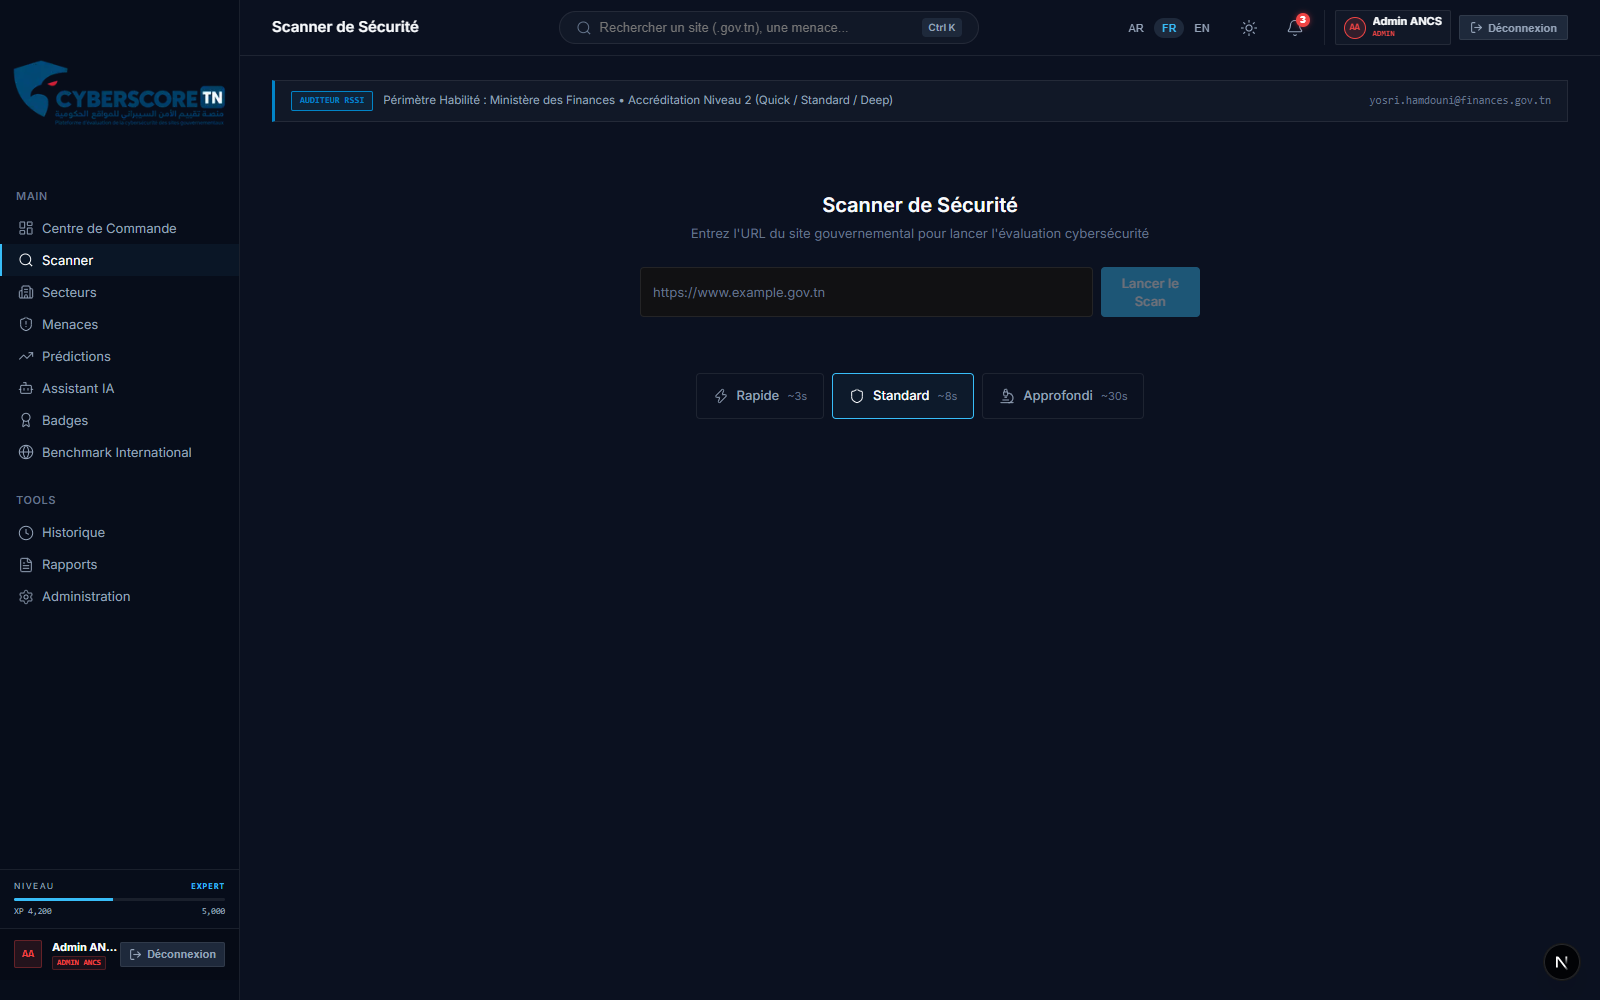
\includegraphics[width=0.70\textwidth]{images/scanner.png}
\caption{Interface d'audit passif et restitution de la fiche technique d'évaluation}
\label{fig:scanner_view}
\end{figure}

\chapter[Scoring \& Classification Sectorielle]{Réalisation : Moteur de Scoring \& Classification Sectorielle}
\label{chap:scoring}

\section{Algorithme Mathématique de Scoring Pondéré}
L'agrégation des résultats d'audit repose sur un modèle mathématique à coefficients pondérés inspiré des meilleures pratiques internationales, mais calibré sur les priorités défensives de l'administration tunisienne.

\subsection{Formule de Calcul}
Soit $N = 16$ l'ensemble des facteurs de risque audités. Pour chaque catégorie $i \in \{1, \dots, N\}$, on note $S_i \in [0, 100]$ le score partiel obtenu et $w_i \in ]0, 1]$ son coefficient de pondération respectif, tel que $\sum_{i=1}^{N} w_i = 1.0$.

Le score global de cybersécurité de l'organisme audité, noté $\text{Score}_{\text{global}} \in [0, 100]$, est défini par la combinaison linéaire normalisée suivante :
\begin{equation}
\text{Score}_{\text{global}} = \sum_{i=1}^{N} \left( w_i \times S_i \right) - \sum_{k \in \mathcal{V}_{\text{critique}}} \mathcal{P}_k
\end{equation}
où $\mathcal{V}_{\text{critique}}$ représente l'ensemble des vulnérabilités critiques rédhibitoires détectées (ex: injection SQL avérée, port de base de données exposé sur Internet sans pare-feu, certificat SSL révoqué), et $\mathcal{P}_k$ une pénalité de sévérité directe (fixée à 15 points par défaut).

\subsection{Grille de Pondération des 16 Facteurs d'Évaluation}
La distribution des poids reflète la criticité opérationnelle des vecteurs d'attaque :

\begin{table}[!htbp]
\centering
\caption{Grille de pondération des 16 facteurs d'audit de CyberScore TN}
\label{tab:weights}
\begin{singlespace}
\footnotesize
\renewcommand{\arraystretch}{1.0}
\begin{tabularx}{\textwidth}{p{4.6cm} c c X}
\toprule
\textbf{Facteur de Risque Audité} & \textbf{Poids} & \textbf{Pts} & \textbf{Justification Opérationnelle} \\
\midrule
Vulnérabilités Web (OWASP ZAP) & 0.15 & 15 & Risque direct d'injections SQL et de compromission. \\
Chiffrement SSL / TLS \& Ciphers & 0.12 & 12 & Confidentialité des flux d'échange citoyen-État. \\
En-têtes HTTP (HSTS / CSP) & 0.10 & 10 & Barrière défensive primaire du navigateur contre les attaques. \\
Sécurité DNS \& DNSSEC & 0.08 & 8 & Protection contre le détournement de trafic et cache poisoning. \\
Exposition Réseau (Ports Nmap) & 0.08 & 8 & Réduction de la surface d'accès aux services internes. \\
Sécurité Email (SPF / DMARC) & 0.06 & 6 & Lutte contre l'usurpation ministérielle et le phishing. \\
Content Security Policy (CSP) & 0.06 & 6 & Atténuation stricte des attaques Cross-Site Scripting (XSS). \\
Sécurité Cookies de Session & 0.05 & 5 & Protection contre le vol de session et détournement. \\
Supply Chain \& CDN (SRI) & 0.05 & 5 & Prévention des attaques par rebond sur dépendances tierces. \\
Fuite d'Infos Techniques (\texttt{.git}) & 0.05 & 5 & Masquage de la topologie interne et des versions serveurs. \\
Surface d'Attaque EASM & 0.04 & 4 & Détection des serveurs fantômes et environnements oubliés. \\
Réputation CTI (Threat Intel) & 0.04 & 4 & Détection des adresses IP compromises et listes noires. \\
Obsolescence des Technologies & 0.03 & 3 & Identification des versions de CMS et logiciels non patchés. \\
Chaîne de Confiance TunTrust & 0.03 & 3 & Souveraineté de l'autorité de certification nationale. \\
Protection Données Privées & 0.03 & 3 & Garantie de non-exposition des données personnelles. \\
Conformité Décret 2023-17 & 0.03 & 3 & Alignement formel sur les directives de sécurité ANCS. \\
\midrule
\textbf{Total National} & \textbf{1.00} & \textbf{100} & \textbf{Évaluation Complète de la Posture Souveraine} \\
\bottomrule
\end{tabularx}
\end{singlespace}
\end{table}

\section{Système de Notation Duale}
Pour répondre à la fois au besoin technique des officiers RSSI et au besoin décisionnel des ministres et directeurs généraux, CyberScore TN propose une notation duale :

\begin{table}[!htbp]
\centering
\caption{Grille de correspondance des Notes, Grades alphabétiques et Étoiles}
\label{tab:grades}
\begin{singlespace}
\footnotesize
\renewcommand{\arraystretch}{1.1}
\begin{tabularx}{\textwidth}{c c c c X}
\toprule
\textbf{Plage de Score} & \textbf{Grade} & \textbf{Étoiles} & \textbf{Mention Officielle} & \textbf{Signification Opérationnelle} \\
\midrule
$95 - 100$ & \textbf{A+} & $\star\star\star$ & Exemplaire & Posture de sécurité optimale, TLS 1.3 et DNSSEC actifs. \\
$90 - 94$  & \textbf{A}  & $\star\star\star$ & Excellent & Très haut niveau de cyber-hygiène, 0 alerte critique. \\
$80 - 89$  & \textbf{B}  & $\star\star\star$ & Bon & Bon niveau global, quelques optimisations recommandées. \\
$70 - 79$  & \textbf{C}  & $\star\star\phantom{\star}$ & Acceptable & Conforme aux standards de base, carences sur HSTS ou CSP. \\
$60 - 69$  & \textbf{D}  & $\star\phantom{\star\star}$ & Insuffisant & Vulnérabilités moyennes nombreuses, remédiation sous 30 jours. \\
$0 - 59$   & \textbf{F}  & $\star\phantom{\star\star}$ & Critique & Présence d'alertes critiques actives, intervention immédiate. \\
\bottomrule
\end{tabularx}
\end{singlespace}
\end{table}

\section{Classification Sectorielle des Organismes Publics Tunisiens}
Afin de structurer le monitoring national, CyberScore TN classe l'ensemble du patrimoine numérique de l'État en quatre secteurs d'activité administrative :
\begin{enumerate}
    \item \textbf{Ministères (24 départements)} : Départements ministériels centraux (\texttt{finances.gov.tn}, \texttt{interieur.gov.tn}, \texttt{defense.nat.tn}, etc.).
    \item \textbf{Institutions Publiques (25+ agences)} : Instances constitutionnelles, agences nationales et régulateurs (\texttt{ancs.tn}, \texttt{bct.gov.tn}, \texttt{isie.tn}, etc.).
    \item \textbf{Collectivités Locales (50+ collectivités)} : Gouvernorats régionaux et municipalités (\texttt{commune-tunis.gov.tn}, \texttt{commune-sfax.gov.tn}, etc.).
    \item \textbf{Entreprises Publiques (20+ sociétés)} : Sociétés d'État et offices publics (\texttt{steg.com.tn}, \texttt{sonede.com.tn}, \texttt{poste.tn}, etc.).
\end{enumerate}

La Figure \ref{fig:benchmark_view} illustre le tableau de bord comparatif permettant à l'ANCS de suivre le niveau moyen de conformité par secteur et d'identifier les organismes nécessitant un appui prioritaire.

\begin{figure}[!htbp]
\centering
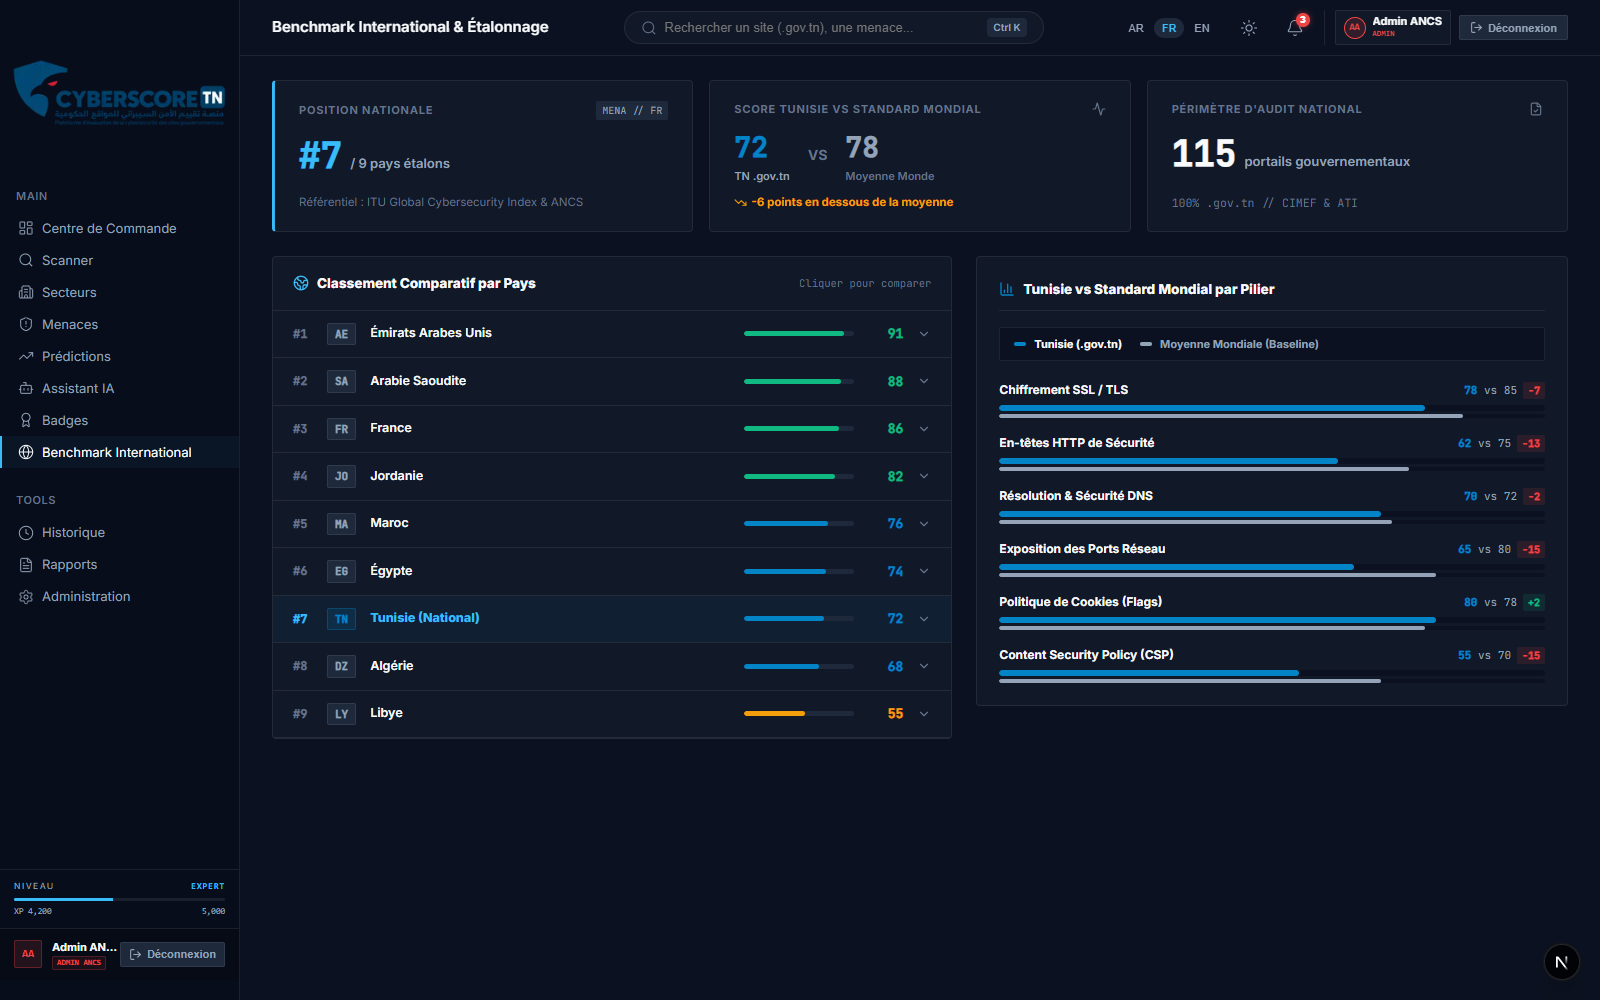
\includegraphics[width=0.70\textwidth]{images/benchmark.png}
\caption{Observatoire comparatif et benchmark sectoriel des institutions d'État}
\label{fig:benchmark_view}
\end{figure}

\section{Modélisation Prédictive des Risques à +30 Jours}
Le moteur analytique corrèle l'historique temporel des audits avec les cycles d'expiration des certificats X.509 et les délais moyens de remédiation observés pour projeter la note de chaque institution à horizon 30 jours (Figure \ref{fig:predictions_view}).

\begin{figure}[!htbp]
\centering
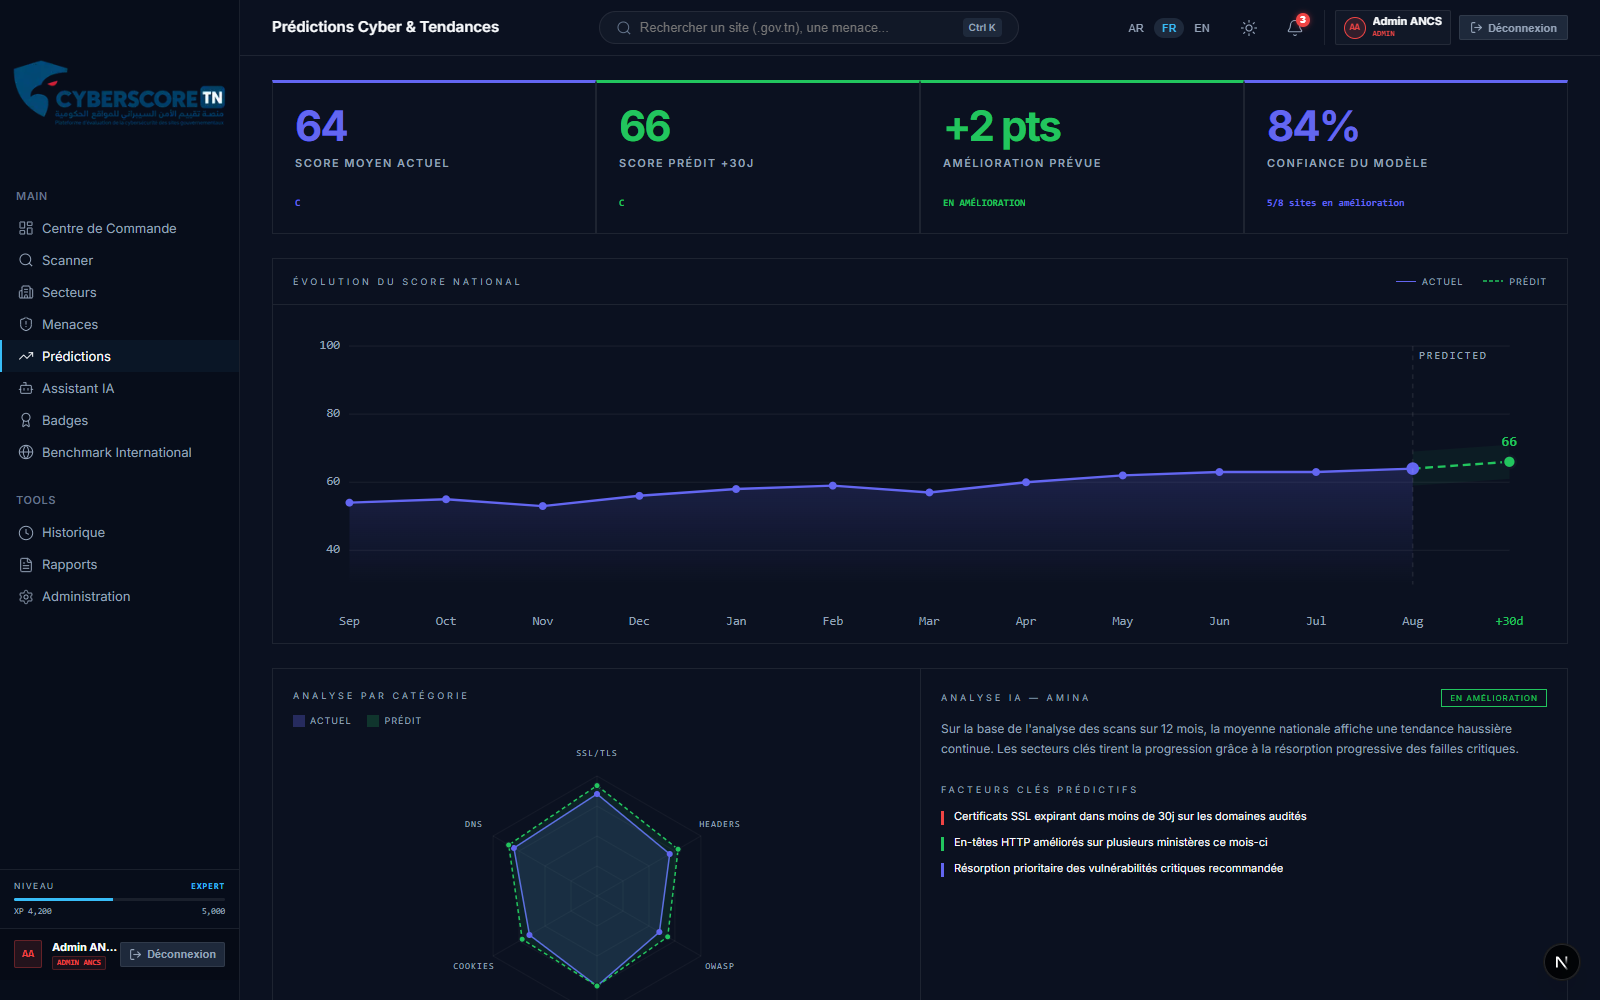
\includegraphics[width=0.70\textwidth]{images/predictions.png}
\caption{Module d'analyse prédictive et projections de dérive de score à +30 jours}
\label{fig:predictions_view}
\end{figure}

\chapter[Interface SOC \& Visualisations]{Réalisation : Interface SOC, Cartographie \& Visualisations}
\label{chap:dashboard}

\section{Design System v2 « Digital Backbone »}
L'interface utilisateur de CyberScore TN a été pensée pour répondre aux standards esthétiques et ergonomiques des postes de commandement de cybersécurité modernes.

\subsection{Palette Chromatique \& Identité Visuelle}
L'ergonomie visuelle repose sur des contrastes élevés adaptés aux longues sessions de supervision :
\begin{itemize}
    \item \textbf{Fond Principal (\texttt{--bg-primary})} : Bleu nuit profond (\texttt{\#04151f}) éliminant la fatigue oculaire.
    \item \textbf{Cartes \& Panneaux (\texttt{--bg-secondary})} : Surface bleu acier sombre (\texttt{\#0a2233}) avec effet de glassmorphism subtil (\texttt{backdrop-filter: blur(8px)}).
    \item \textbf{Accent Principal (\texttt{--color-primary})} : Cyan électrique (\texttt{\#00e5ff}) pour les éléments actifs et trajectoires.
    \item \textbf{Codes de Sévérité Universels} : Vert émeraude (\texttt{\#00e676}) pour les postures excellentes, ambre (\texttt{\#ffb300}) pour les alertes modérées, et rouge écarlate (\texttt{\#ff1744}) pour les failles critiques.
\end{itemize}

\section{Centre de Commande National (Command Center)}
Le Command Center (\texttt{/}) rassemble l'ensemble des flux télémétriques de l'État :
\begin{enumerate}
    \item \textbf{StatCards Connectées en Temps Réel} : Affichage dynamique des quatre indicateurs clés de performance : nombre d'institutions sous surveillance active (121 sites gouvernementaux), score moyen national consolidé (57.6/100), alertes critiques réelles détectées (112) et volume des scans effectués dans la journée.
    \item \textbf{Leaderboard National \& Modal d'Aperçu Interactif} : Tableau de classement trié par note. Un clic sur n'importe quel organisme ouvre instantanément une visionneuse interactive de 7 pages (\texttt{ReportPreviewModal.tsx}) affichant la synthèse exécutive, l'analyse radar et les vulnérabilités détectées.
\end{enumerate}

\subsection{Recalibrage Géométrique SVG de la Carte de Tunisie}
L'affichage cartographique régional présentait initialement un rognage sur le gouvernorat de Tataouine et les côtes de Djerba. Une analyse trigonométrique des coordonnées des 24 gouvernorats a permis d'établir l'emprise géographique réelle :
\begin{itemize}
    \item \textbf{Axe horizontal} : De $X = 289.5$ (Tozeur / frontière ouest) à $X = 710.5$ (Djerba / côtes est), soit une largeur de 421.0 px.
    \item \textbf{Axe vertical} : De $Y = 45.5$ (Bizerte / Cap Blanc) à $Y = 954.5$ (Borj El Khadra / pointe sud), soit une hauteur de 909.0 px.
\end{itemize}
Le composant vectoriel SVG a été calibré avec la \texttt{viewBox} optimale :
\begin{lstlisting}[language=XML, caption={Recalibrage du composant vectoriel de la carte de Tunisie}]
<svg id="tn-map" viewBox="275 35 450 935" xmlns="http://www.w3.org/2000/svg">
\end{lstlisting}
Chaque gouvernorat est coloré dynamiquement en fonction du score moyen des sites rattachés à sa circonscription administrative (Figure \ref{fig:dashboard_view}).

\begin{figure}[!htbp]
\centering
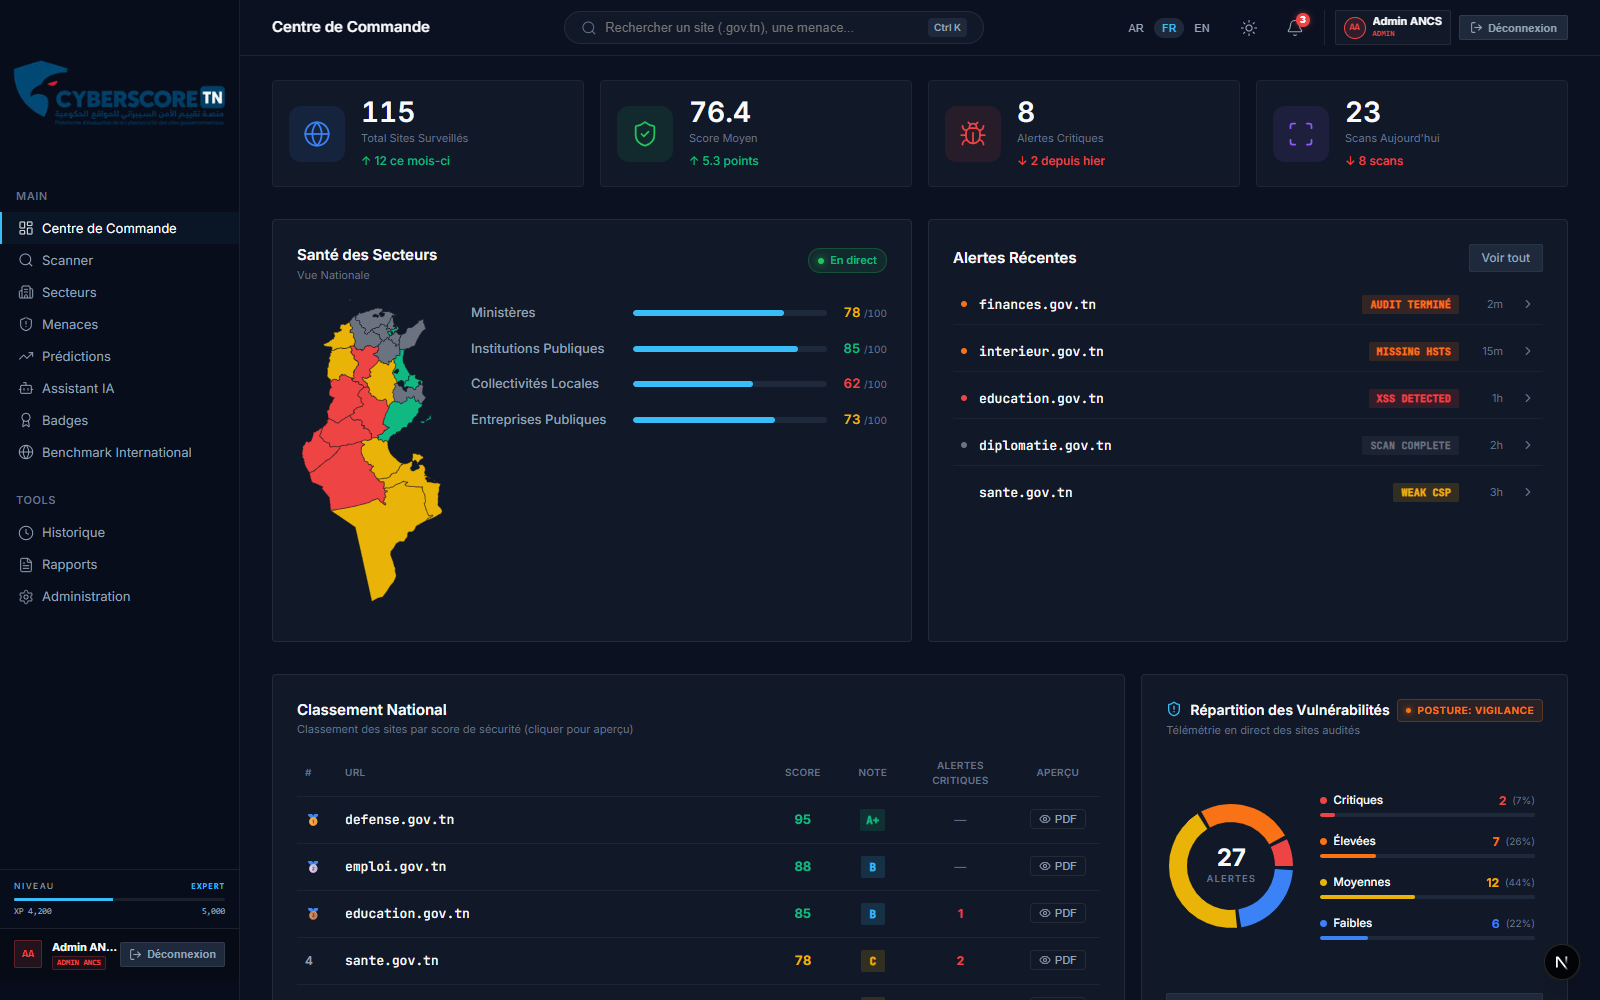
\includegraphics[width=0.70\textwidth]{images/dashboard.png}
\caption{Tableau de bord national (Command Center) et cartographie vectorielle interactive}
\label{fig:dashboard_view}
\end{figure}

\section{Observatoire de Benchmark International \& Étalonnage (\texttt{/benchmark})}
L'Observatoire International permet de situer la posture nationale de la Tunisie par rapport aux standards mondiaux et aux pays pairs de la région MENA et d'Europe :
\begin{itemize}
    \item \textbf{Calcul Dynamique en Temps Réel} : Contrairement aux approches statiques, la position de la Tunisie est recalculée dynamiquement à partir des audits réels des 121 portails gouvernementaux et des scans interactifs.
    \item \textbf{Étalonnage par Piliers Techniques} : Comparaison fine sur six axes cruciaux : chiffrement SSL/TLS, en-têtes HTTP de sécurité, sécurité DNS/DNSSEC, exposition des ports réseau, politique de cookies et Content Security Policy (CSP).
    \item \textbf{Synchronisation Réactive} : Tout audit réalisé dans le scanner met instantanément à jour le score national et le classement comparatif.
\end{itemize}

\section{War Room \& Mappemonde Cyber Animée (\texttt{/threats})}
La page de surveillance des cybermenaces propose une tour de contrôle combinant audits réels et télémétrie mondiale (CTI) :
\begin{itemize}
    \item \textbf{Moteur Graphique Canvas 60 FPS} : Rendu fluide affichant les trajectoires balistiques d'attaques mondiales modélisées par des courbes de Bézier quadratiques convergeant vers les coordonnées géographiques de la Tunisie (33.88\textdegree{} N, 9.53\textdegree{} E).
    \item \textbf{Effets d'Impact \& Détection de Collision} : Les flux interceptés par les pare-feu périmétriques déclenchent un flash visuel au point d'impact.
    \item \textbf{Cartes Hybrides des Vulnérabilités (CVEs)} : Affichage prioritaire des failles critiques réelles identifiées lors des scans de nos serveurs étatiques, complété par un flux de renseignement mondial sur les menaces émergentes.
\end{itemize}

\begin{figure}[!htbp]
\centering
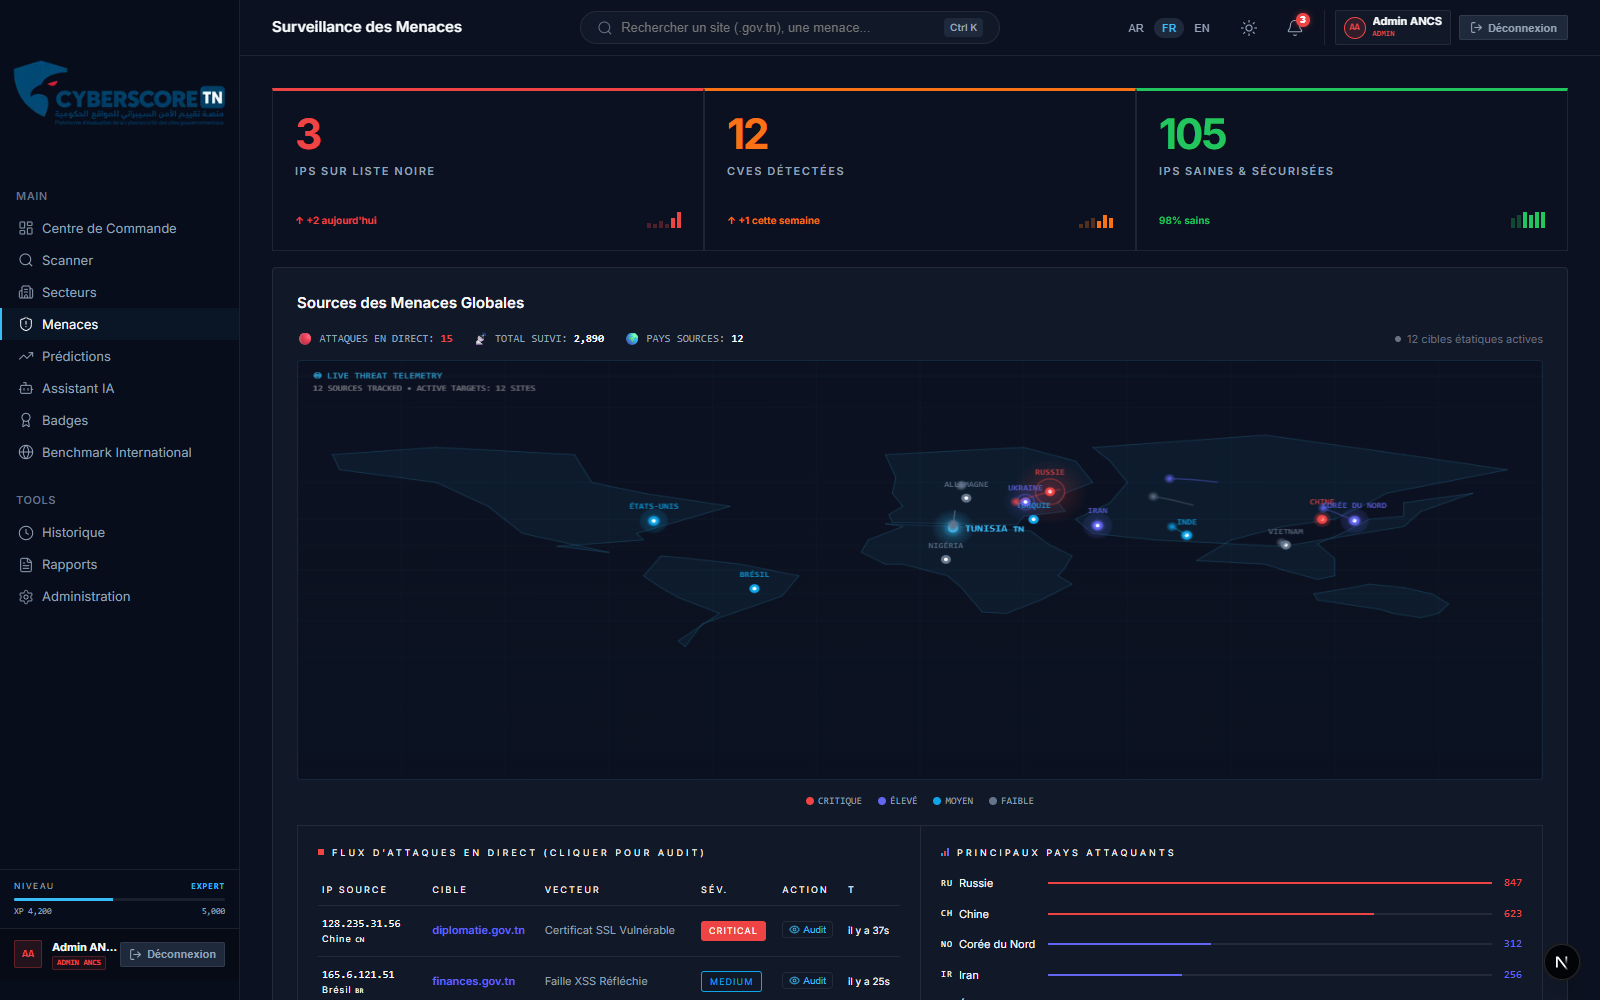
\includegraphics[width=0.70\textwidth]{images/threats.png}
\caption{War Room souveraine et flux mondial des cyberattaques en temps réel (Canvas 60 FPS)}
\label{fig:threats_view}
\end{figure}

\section{Centre National d'Édition des Rapports d'Audit (\texttt{/reports})}
Le module de reporting certifié permet d'exporter des fiches d'audit et des attestations officielles au format PDF vectoriel haute résolution. Chaque rapport intègre :
\begin{itemize}
    \item \textbf{Cartouche Officiel de Conformité ANCS} : Mention du Décret-loi n° 2023-17 et classification TLP.
    \item \textbf{Visualisation Radar des 16 Piliers} : Graphique vectoriel A4 illustrant la posture technique relative.
    \item \textbf{Signature Numérique SHA-256 \& QR Code} : Empreinte cryptographique certifiant l'intégrité du document sans altération (Figure \ref{fig:reports_view}).
\end{itemize}

\begin{figure}[!htbp]
\centering
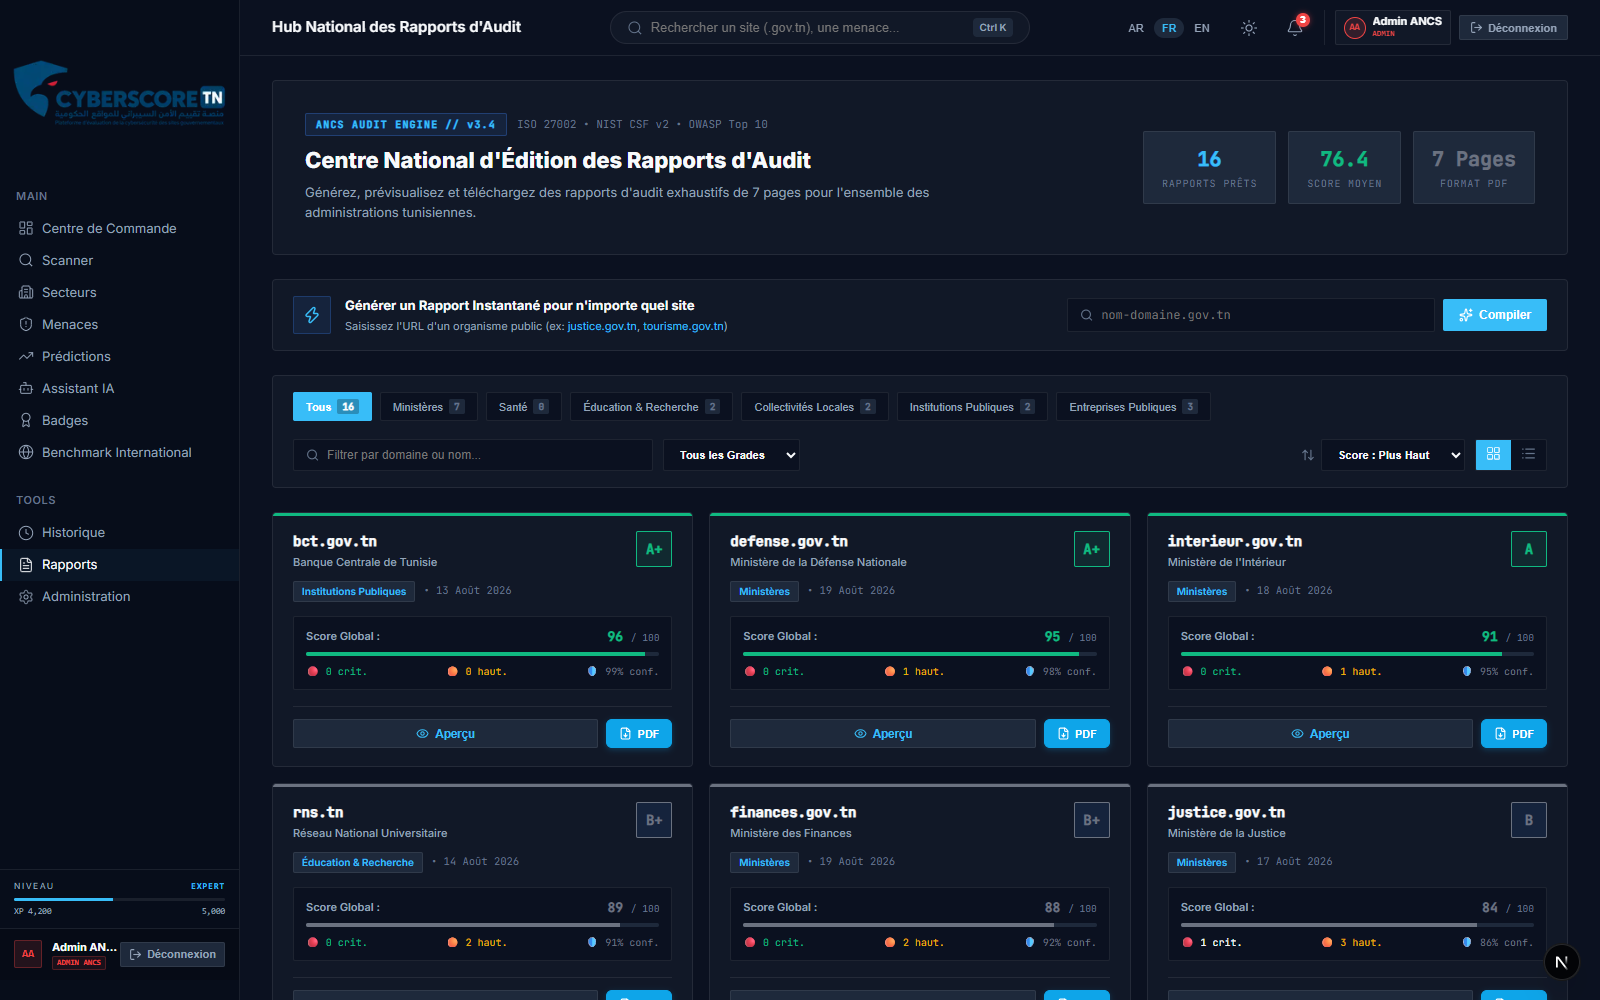
\includegraphics[width=0.70\textwidth]{images/reports.png}
\caption{Centre d'édition des rapports d'audit officiels et d'attestations de conformité}
\label{fig:reports_view}
\end{figure}

\chapter[IA Souveraine \& Avatar 3D]{Réalisation : Intelligence Artificielle Souveraine \& Avatar 3D}
\label{chap:ia}

\section{Architecture du LLM Souverain Qwen2.5-Coder:7b}
L'un des défis majeurs pour les infrastructures d'État consiste à bénéficier des capacités de pointe de l'IA générative sans compromettre la souveraineté des données.

\subsection{Spécifications du Modèle \& Runtime Ollama}
CyberScore TN intègre le modèle de fondation \textbf{\texttt{Qwen2.5-Coder:7b}} (format quantifié GGUF Q4\_K\_M, empreinte mémoire de 4.7 Go), exécuté localement via le runtime Ollama sur le port \texttt{25000} (avec fallback sur le port par défaut \texttt{11434}) :
\begin{itemize}
    \item \textbf{Performance de Génération de Code} : Score de 88.4\% au benchmark HumanEval, surpassant la majorité des modèles de sa catégorie et rivalisant avec GPT-4o sur la production de configurations de sécurité (fichiers \texttt{nginx.conf}, directives Apache, règles \texttt{nftables}, scripts Bash de durcissement).
    \item \textbf{Souveraineté Intégrale \& Zéro Fuite Cloud} : Aucune configuration serveur, aucune adresse IP et aucun descriptif de vulnérabilité ne quitte l'infrastructure matérielle locale.
\end{itemize}

\subsection{Flux Streaming Direct en Temps Réel (Server-Sent Events)}
Pour éliminer les temps de latence perceptibles par l'utilisateur, l'échange avec le modèle utilise le protocole de streaming SSE (\textit{Server-Sent Events}). Les jetons textuels générés sont poussés mot-par-mot vers le navigateur avec une cadence de 60 FPS, offrant une sensation d'élocution naturelle.

\begin{figure}[!htbp]
\centering
\begin{tcolorbox}[colback=white,colframe=tekupPurple,arc=0mm,title=\textbf{Flux Asynchrone de Streaming Navigateur $\leftrightarrow$ IA Locale}]
\small
\begin{enumerate}
    \item L'officier RSSI transmet sa question technique ou clique sur une suggestion contextuelle.
    \item L'interface Next.js émet une requête \texttt{POST /api/chat} avec le paramètre \texttt{stream: true} vers le backend ou le runtime local.
    \item \textbf{Mode Nominal (Ollama en ligne)} : Ollama génère la réponse et renvoie les tokens en continu (SSE). L'avatar Three.js synchronise ses mouvements d'élocution.
    \item \textbf{Mode Dégradé (Fallback Hors-Ligne)} : Si le port de l'IA est inaccessible, le système active instantanément un générateur expert déterministe certifié ANCS qui restitue les directives de durcissement adaptées sans interruption de service.
\end{enumerate}
\end{tcolorbox}
\caption{Schéma du flux conversationnel avec basculement résilient automatique}
\label{fig:flow_ia}
\end{figure}

\section{Avatar 3D Haute Définition « Amina »}
L'assistance cyber s'incarne sous la forme de l'avatar 3D \textbf{Amina} (\texttt{AminaAvatar3D.tsx}) :
\begin{itemize}
    \item \textbf{Moteur de Rendu Three.js / React Three Fiber} : Modèle 3D optimisé intégrant des animations faciales synchronisées selon l'état de réflexion (\textit{mood: thinking}) et de parole (\textit{isTalking: true}).
    \item \textbf{Cartouche d'Identification SOC Glassmorphism} : Plaque d'identification en verre fumé avec liseré cyan électrique mentionnant \textbf{AMINA -- AI SECURITY ANALYST} (Figure \ref{fig:avatar_view}).
\end{itemize}

\begin{figure}[!htbp]
\centering
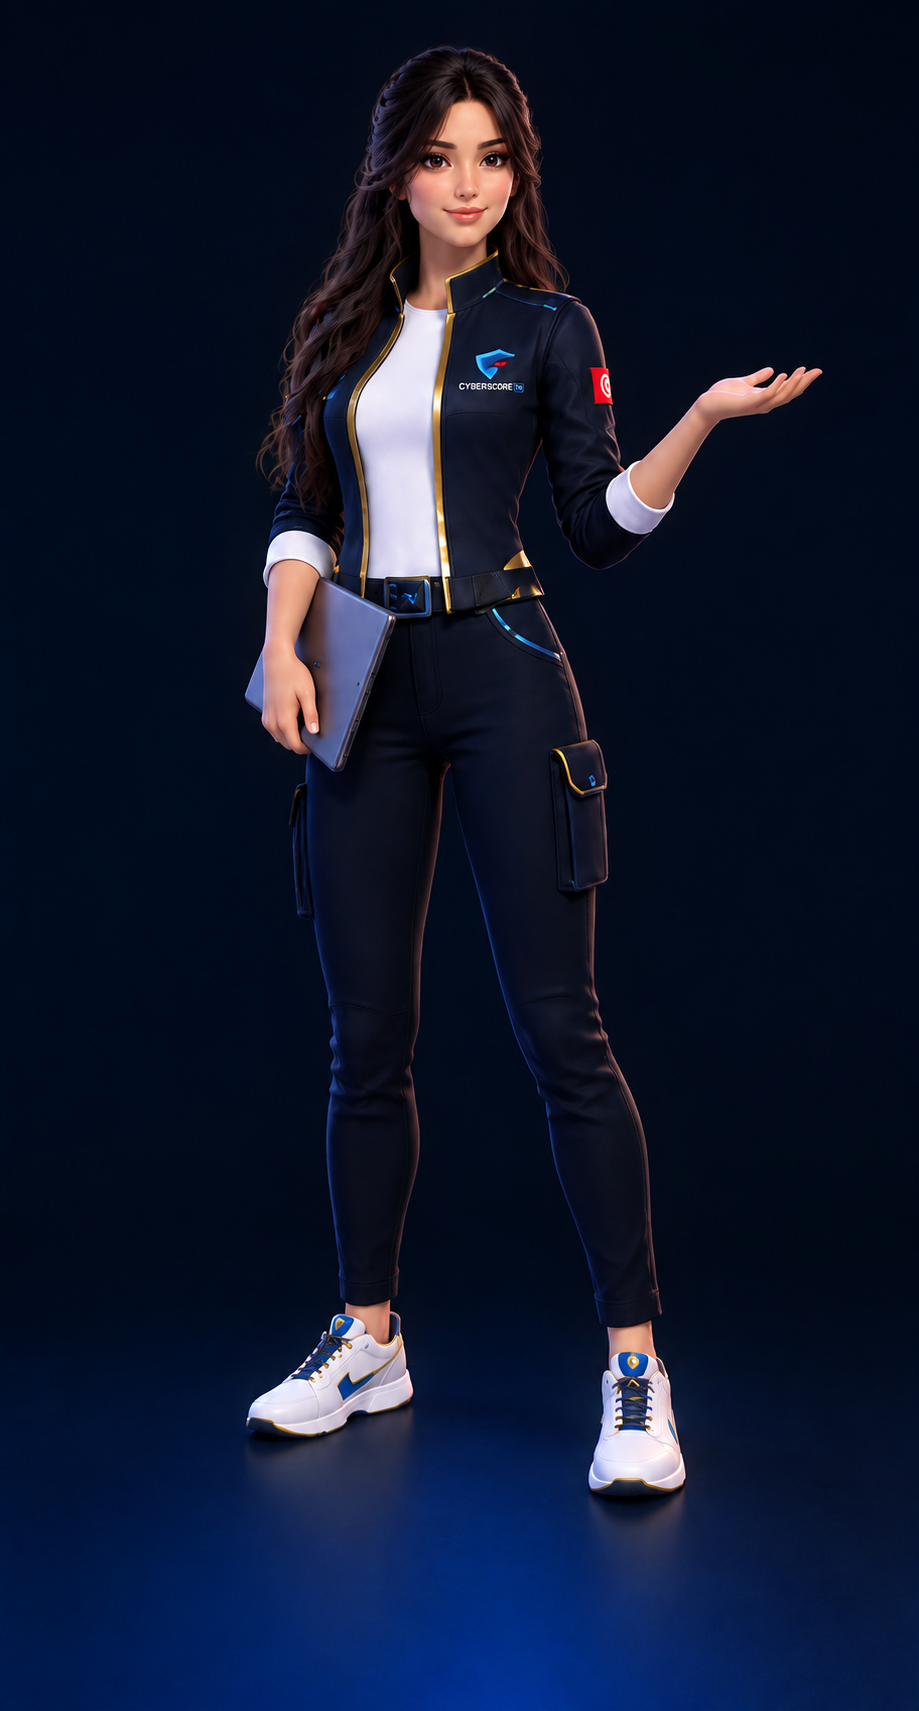
\includegraphics[height=6cm, keepaspectratio]{images/avatar_amina.png}
\caption{Modélisation visuelle de l'analyste IA souveraine Amina}
\label{fig:avatar_view}
\end{figure}

\section{Console SOC Interactive \& Contrôle de Session}
La console conversationnelle intègre des fonctionnalités avancées de gestion de cycle de vie :
\begin{enumerate}
    \item \textbf{Persistance Automatique de l'Historique} : Sérialisation continue des échanges dans le stockage local du navigateur (\texttt{localStorage}). L'auditeur peut naviguer librement entre les différentes pages de la plateforme sans perdre le fil de son échange.
    \item \textbf{Bouton d'Arrêt d'Urgence (\texttt{AbortController})} : Pendant la génération du flux par le modèle, le bouton d'envoi bascule dynamiquement en interrupteur rouge \textbf{STOP}. Un clic déclenche l'interruption immédiate de la requête HTTP sans geler l'interface.
    \item \textbf{Suggestions 1-Clic Contextuelles} : Bandeau de raccourcis rapides adaptés aux rôles opérationnels (diagnostic de score pour les analystes SOC, configurations Nginx pour les ingénieurs système, plan d'action à 30 jours pour les RSSI, et synthèse exécutive non-technique pour la direction générale).
    \item \textbf{Synchronisation Dynamique Multi-Scans \& Éradication du Cache Périmé} : Propagation automatique des métriques réelles d'audit (\texttt{score}, \texttt{grade}, décompte exact des vulnérabilités) depuis les 4 modes de scan (Quick, Standard, Deep, Autonome IA) vers l'assistant IA, avec renouvellement automatique de l'historique obsolète pour garantir une parfaite cohérence entre le rapport d'audit et le premier message d'orientation.
\end{enumerate}

La Figure \ref{fig:assistant_view} présente l'interface opérationnelle de l'assistant IA, illustrant la génération dynamique de remédiations techniques sans aucune fuite cloud.

\begin{figure}[!htbp]
\centering
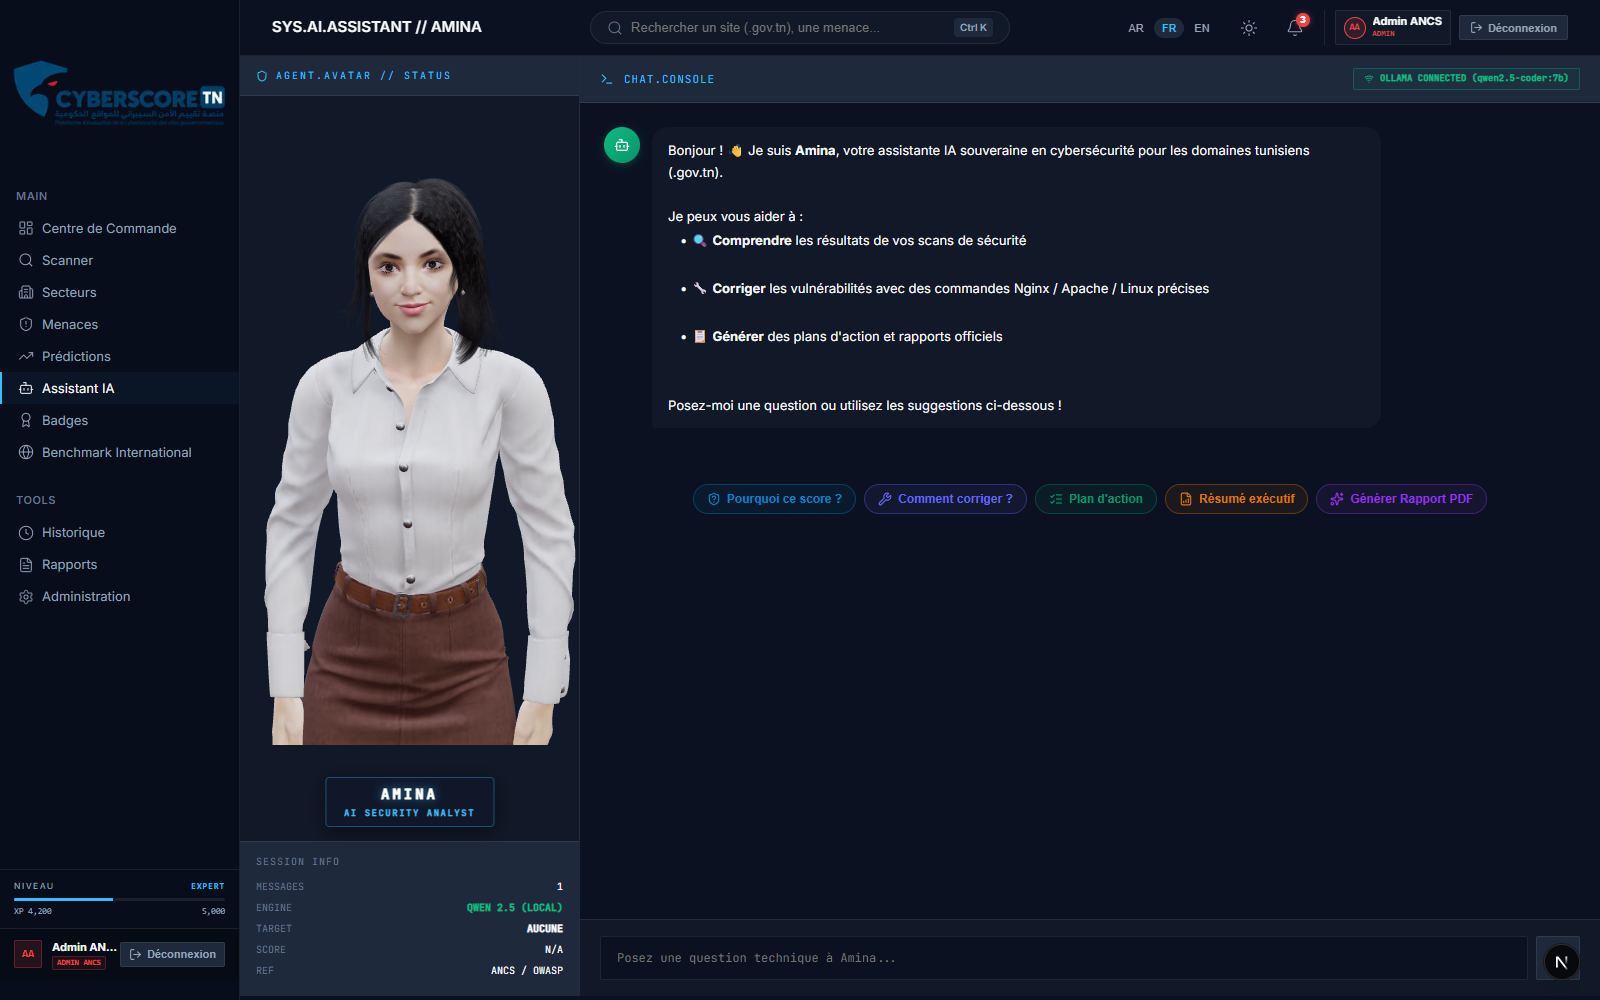
\includegraphics[width=0.70\textwidth]{images/assistant.png}
\caption{Console conversationnelle de l'analyste IA Amina sous Qwen2.5-Coder:7b}
\label{fig:assistant_view}
\end{figure}

\chapter[Sécurité RBAC \& Gamification]{Réalisation : Sécurité RBAC, Gamification \& Sceau Public}
\label{chap:backend_gamification}

\section{Contrôle d'Accès Basé sur les Rôles (RBAC) \& Sécurité JWT}
Dans un environnement étatique sensible, la compartimentation des privilèges est indispensable pour empêcher les accès non autorisés et garantir la traçabilité des opérations d'audit.

\subsection{Matrice des Privilèges \& Hachage Bcrypt}
L'authentification s'appuie sur des jetons \textbf{JSON Web Tokens (JWT)} signés cryptographiquement en \textbf{HMAC-SHA256} avec durée de validité restreinte. Les mots de passe en base sont irréversiblement protégés par l'algorithme \textbf{Bcrypt} (facteur de coût 12). Les rôles sont cloisonnés selon trois niveaux d'autorité :
\begin{itemize}
    \item \textbf{\texttt{Admin} (Super-Admin ANCS)} : Supervision globale des 120 institutions, gestion des comptes utilisateurs, validation des habilitations ministérielles, accès exclusif à la console \texttt{/admin}, édition dynamique du registre des organisations (criticité 1 à 5, contact CSIRT, périmètre surveillé) et activation du mode maintenance.
    \item \textbf{\texttt{Auditor} (Officier RSSI Ministériel)} : Accrédité sur son périmètre ministériel dédié (ex: Ministère des Finances), habilité à déclencher des scans approfondis, à interagir avec l'IA Amina et à exporter les rapports officiels PDF. Toute tentative d'accès à \texttt{/admin} ou de modification du registre étatique est interceptée et bloquée.
    \item \textbf{\texttt{Viewer} (Observateur Public)} : Consultation en lecture seule des scores agrégés et du benchmark international. Les boutons de lancement d'audit, les fonctions de modification et la console d'administration lui sont strictement inaccessibles.
\end{itemize}

\subsection{Écran de Sécurité Souverain HTTP 403 Forbidden sur \texttt{/admin}}
Toute tentative d'accès à la route d'administration par un profil non habilité est stoppée au niveau du routeur Next.js et de l'API FastAPI. L'interface affiche un écran de sécurité haute visibilité rappelant la règle de moindre privilège et journalise la tentative dans l'Audit Trail pour inspection par l'ANCS (Figure \ref{fig:admin_view}).

\subsection{Gestion Dynamique des Organisations \& Privilèges Super-Admin Exclusifs}
Afin de refléter l'évolution des infrastructures publiques sans nécessiter de redéploiement backend, la console d'administration permet la mise à jour en direct du registre des 24 ministères et entités étatiques :
\begin{itemize}
    \item \textbf{Édition directe en ligne} : Modification du niveau de criticité nationale (échelle de 1 à 5 barres selon l'impact souverain), mise à jour de l'adresse de contact d'urgence CSIRT, et enrôlement de nouvelles structures ministérielles.
    \item \textbf{Privilèges strictement réservés au rôle \texttt{admin}} : Ces capacités de mutation sont verrouillées au niveau de l'interface et protégées par des contrôles d'habilitation programmatiques (\texttt{loggedUser.role === "admin"}). Tout profil non-admin est stoppé par une interdiction HTTP 403.
    \item \textbf{Imputabilité \& Audit Trail en temps réel} : Chaque modification ou enrôlement d'institution génère un enregistrement immédiat et infalsifiable dans le flux d'audit (\texttt{LIVE FEED}) avec horodatage à la seconde, garantissant la conformité au Décret-loi n° 2023-17.
\end{itemize}

\begin{figure}[!htbp]
\centering
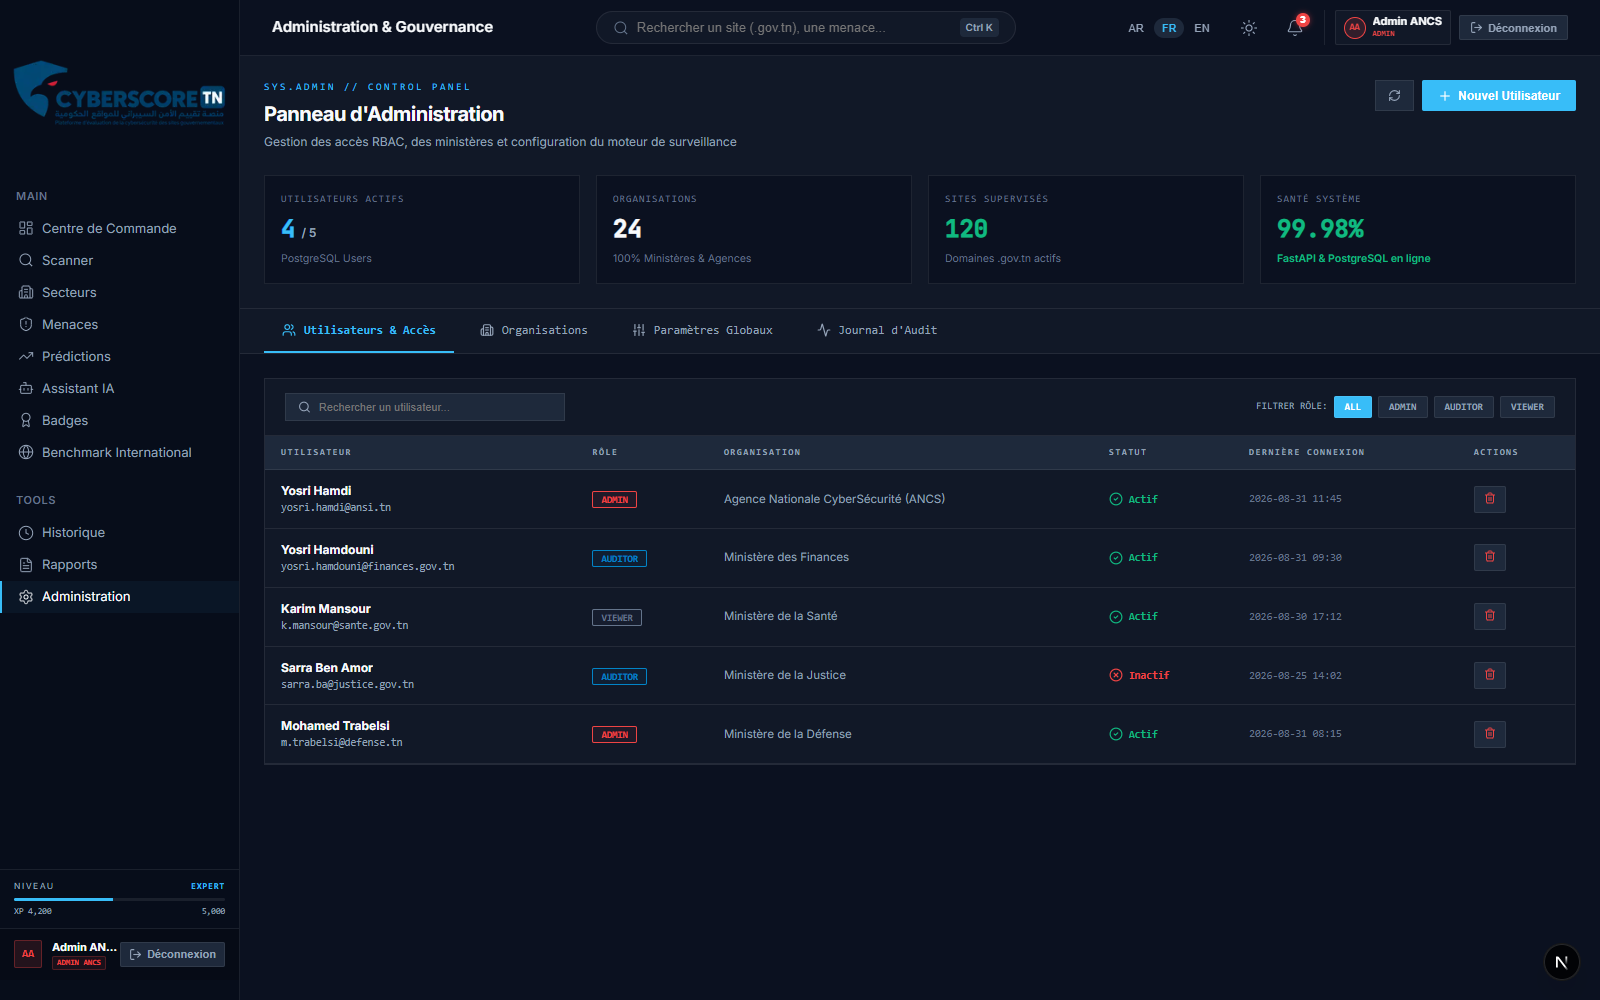
\includegraphics[width=0.70\textwidth]{images/admin.png}
\caption{Console d'administration sécurisée et écran de protection RBAC HTTP 403 Forbidden}
\label{fig:admin_view}
\end{figure}

\section{Module de Gamification Institutionnelle \& Niveaux RSSI}
Afin d'inciter les départements ministériels à corriger activement leurs vulnérabilités, CyberScore TN intègre un système d'émulation basé sur l'attribution de points d'expérience (\textbf{XP}).

\subsection{Paliers de Compétence SOC}
L'officier RSSI progresse à travers cinq échelons de reconnaissance affichés dans la barre latérale :
\begin{enumerate}
    \item \textbf{Niveau 1 -- DÉBUTANT ($0 - 1\,000$ XP)} : Prise en main et premiers scans réalisés.
    \item \textbf{Niveau 2 -- INTERMÉDIAIRE ($1\,000 - 2\,000$ XP)} : Audits réguliers du périmètre ministériel.
    \item \textbf{Niveau 3 -- AVANCÉ ($2\,000 - 3\,500$ XP)} : Résolution active des alertes critiques et durcissement SSL/DNS.
    \item \textbf{Niveau 4 -- EXPERT ($3\,500 - 5\,000$ XP)} : Maintien continu du parc au Grade A/A+ et exports officiels.
    \item \textbf{Niveau 5 -- ÉLITE SOC ($5\,000+$ XP)} : Posture exemplaire sur l'ensemble des 16 piliers d'audit.
\end{enumerate}

\subsection{Référentiel des 12 Badges d'Excellence}
Le système évalue automatiquement les métriques enregistrées en base pour attribuer douze trophées officiels aux officiers de sécurité et aux organismes :

\begin{table}[!htbp]
\centering
\caption{Catalogue officiel des 12 badges d'émulation de CyberScore TN}
\label{tab:gamification_badges}
\begin{singlespace}
\footnotesize
\renewcommand{\arraystretch}{1.08}
\begin{tabularx}{\textwidth}{l l c X}
\toprule
\textbf{Code Badge} & \textbf{Intitulé Officiel} & \textbf{XP} & \textbf{Condition de Déblocage Vérifiée} \\
\midrule
\texttt{FIRST\_SCAN} & Premier Pas & +100 & Réalisation du premier audit sur un portail public. \\
\texttt{WARRIOR} & Guerrier de la Sécurité & +250 & Audit complété sur dix domaines étatiques distincts. \\
\texttt{CLEAN\_SWEEP} & Nettoyage Total & +300 & Élimination de toute vulnérabilité critique sur le parc. \\
\texttt{SSL\_CHAMP} & Champion TLS & +250 & Note parfaite de 100/100 sur le pilier SSL/TLS (TLS 1.3). \\
\texttt{HEADERS\_HERO} & Héros des Headers & +250 & Note de 100/100 sur les en-têtes HTTP de sécurité. \\
\texttt{DNS\_GUARD} & Gardien DNS & +200 & Validation DNSSEC et conformité DMARC (\texttt{p=reject}). \\
\texttt{CENTURION} & Centurion du SOC & +500 & Atteinte du seuil de 100 sessions d'audit conduites. \\
\texttt{SECTOR\_LEAD} & Leader Sectoriel & +400 & Première place obtenue au classement du secteur ministériel. \\
\texttt{FAST\_PATCH} & Chasseur de Failles & +350 & Résolution vérifiée d'une faille critique sous 24 heures. \\
\texttt{TRUST\_SEAL} & Sceau de Confiance & +400 & Attribution officielle du label de confiance 3 étoiles. \\
\texttt{VELOCITY} & Audit Véloce & +150 & Audit Standard exécuté avec succès en moins de 5 secondes. \\
\texttt{PERFECTION} & Perfection Nationale & +1\,200 & Score d'audit parfait de 100/100 en mode Approfondi. \\
\bottomrule
\end{tabularx}
\end{singlespace}
\end{table}

La Figure \ref{fig:badges_view} illustre la console d'émulation présentant les paliers de points d'expérience et l'état de déblocage des trophées pour l'organisme audité.

\begin{figure}[!htbp]
\centering
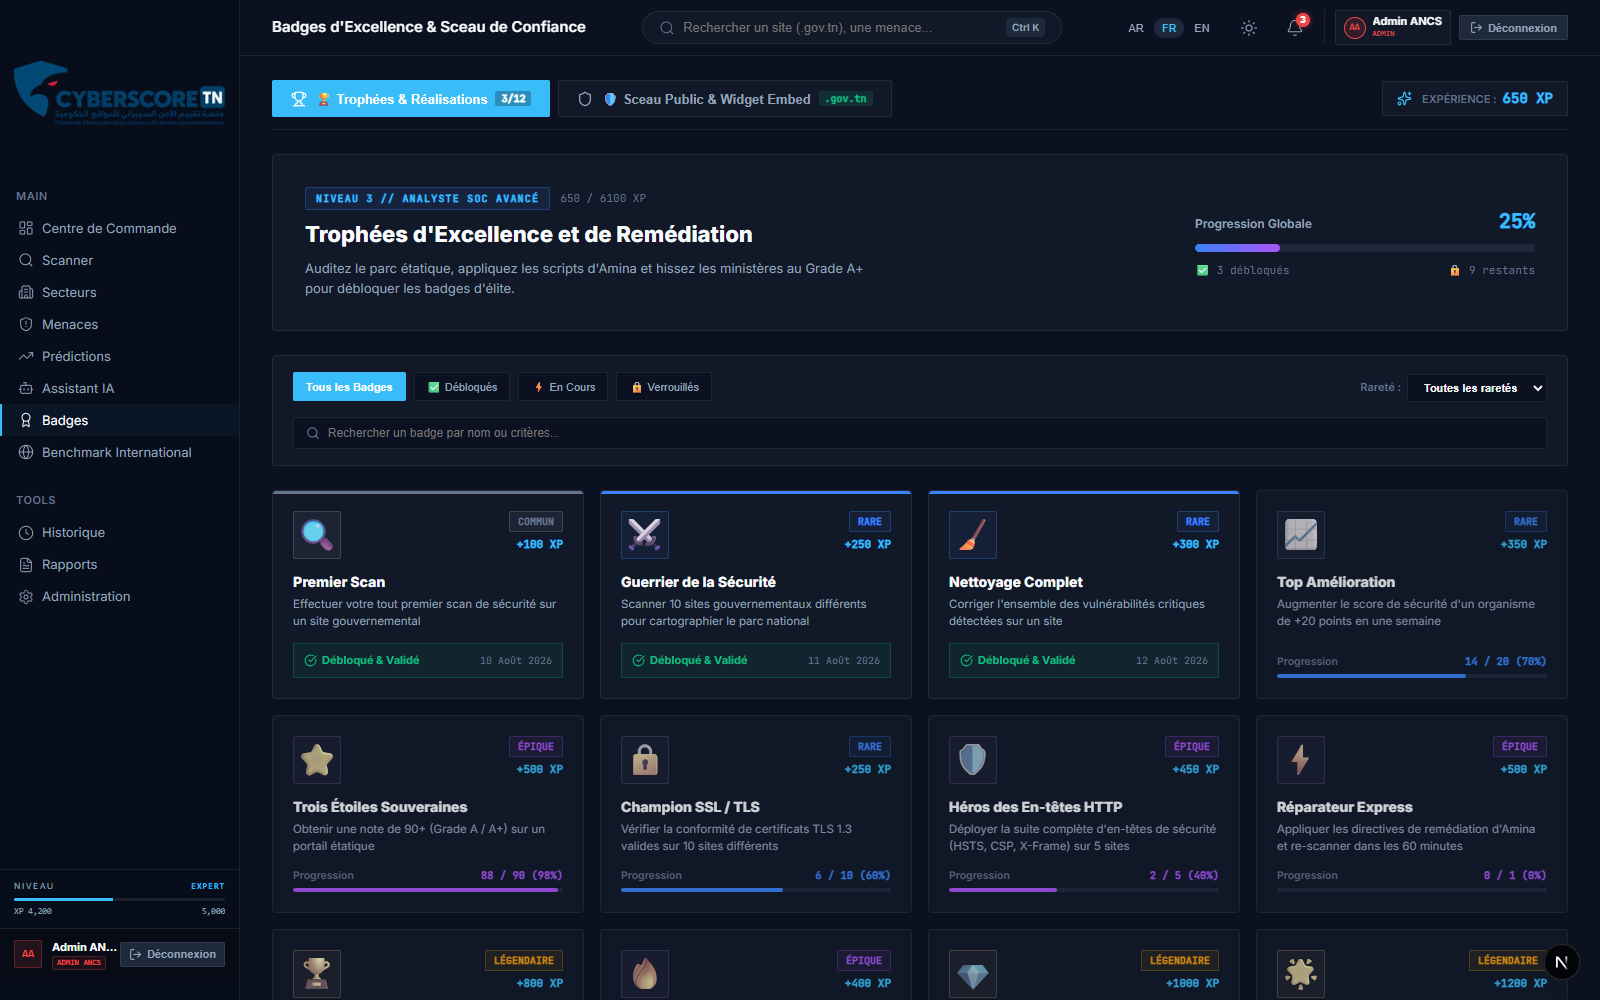
\includegraphics[width=0.70\textwidth]{images/badges.png}
\caption{Centre d'émulation institutionnelle et catalogue interactif des 12 badges SOC}
\label{fig:badges_view}
\end{figure}

\section{Sceau Public de Confiance \& Widget SVG Sécurisé}
Pour valoriser les efforts de mise en conformité auprès du grand public, les organismes atteignant l'excellence peuvent exporter le \textbf{Sceau Numérique de Confiance CyberScore TN} :
\begin{itemize}
    \item \textbf{Widget Vectoriel Dynamique} : Badge SVG auto-actualisé affichant le grade souverain (\texttt{A+}, \texttt{A}, \texttt{B}) et le label d'étoiles ($\star\star\star$).
    \item \textbf{QR Code Anti-Fraude} : Chaque badge embarque un QR code dynamique généré côté client et serveur pointant vers l'URL officielle de vérification cryptographique (\texttt{https://cyberscore.tn/[locale]/verify/[domaine]}), interdisant l'usage frauduleux d'une image statique par un portail non certifié.
    \item \textbf{Variantes d'Intégration} : Cartouche complet institutionnel (armoiries, note, étoiles et QR code), bouclier vertical (\textit{Shield}) et bandeau compact (\textit{Pill}) pour pieds de page.
\end{itemize}

\section{Portail Souverain de Vérification \& Hygiène Numérique Citoyenne}
Afin de concrétiser la vérification par smartphone accessible à tout citoyen, nous avons conçu la route dynamique \texttt{/[locale]/verify/[domain]} :
\begin{enumerate}
    \item \textbf{Architecture Trilingue Réactive} : Prise en charge native de l'Arabe (\textit{RTL}), du Français et de l'Anglais (\textit{LTR}) avec commutation instantanée sans rechargement de page et protection stricte contre les conflits d'hydratation (\texttt{suppressHydrationWarning}).
    \item \textbf{Cloisonnement Défensif TLP:AMBER+STRICT} : L'usager public accède à la certification macroscopique, au score et aux étoiles sans pouvoir consulter les données offensives d'audit. Le rapport technique complet de 7 pages (détaillant les CVE, ports ouverts et snippets de correction) ainsi que le déclencheur de re-scan sont strictement verrouillés derrière une authentification forte réservée aux RSSI accrédités de l'ANCS.
    \item \textbf{Carrousel Héroïque d'Hygiène Numérique} : Un slider interactif animé à rotation automatique (5,5s) avec pause au survol présente les 4 réflexes vitaux de cyber-vigilance : vérification du cadenas HTTPS et du domaine officiel \texttt{.gov.tn}, alerte anti-phishing et faux SMS, activation de l'authentification à double facteur (2FA), et signalement d'urgence auprès du CERT National (ANCS) via le numéro d'urgence \texttt{71 843 200}.
\end{enumerate}

\section{Modélisation des Menaces \& Résilience Face au Phishing (Anti-Phishing)}
Une question déterminante de sécurité offensive s'impose lors de l'évaluation du système : \textit{« Un cybercriminel peut-il capturer le QR code officiel d'un ministère et le publier sur son faux site pour abuser la confiance des citoyens ? »}

Notre réponse technique neutralise cette menace par \textbf{trois lignes de défense coordonnées} basées sur le principe de \textbf{Liaison de Domaine (Domain Binding)} :
\begin{enumerate}
    \item \textbf{Le Piège de Non-Concordance de Domaine (Domain Mismatch Trap)} : Le QR code encode exclusivement l'URL officielle certifiée de l'État (\texttt{cyberscore.tn/verify/sante.gov.tn}). Lorsque la victime scanne le QR code volé depuis un faux portail (\texttt{sante-fake-tunisie.com}), son smartphone ouvre la page souveraine de l'ANCS affichant en gros caractères officiels : \textit{« Cette attestation appartient exclusivement au Ministère de la Santé (sante.gov.tn) »}. La victime constate la divergence flagrante avec l'adresse affichée sur son ordinateur : l'escroquerie est démasquée en une seconde. La capture du QR code devient ainsi le piège qui confond l'attaquant.
    \item \textbf{Ancrage d'Infrastructure Souveraine .tn \& TunTrust} : Un fraudeur ne peut enregistrer de domaine officiel sous la zone étatique \texttt{.tn} (régulée par l'ATI et l'ANCS), ni obtenir un certificat serveur officiel TunTrust sous le backbone AS2609. S'il tente de faire auditer son faux domaine sur la plateforme CyberScore TN, les 6 moteurs de scan passif détectent immédiatement l'absence d'infrastructure nationale et lui attribuent la note éliminatoire de \textbf{Grade F (0/100) — DOMAINE SUSPECT}.
    \item \textbf{Validation Dynamique d'Origine (HTTP Referer \& Hostname)} : Le widget JavaScript (\texttt{BadgesClient.tsx}) vérifie à l'exécution le nom d'hôte (\texttt{window.location.hostname}) et l'en-tête \texttt{Referer}. En cas d'appel depuis un domaine non répertorié dans la base nationale, le serveur révoque l'affichage du sceau de confiance au profit d'un avertissement d'invalidité.
\end{enumerate}


\chapter[Tests \& Validation Expérimentale]{Tests, Métriques \& Validation Expérimentale}
\label{chap:tests}

\section{Stratégie de Test Multi-Niveaux}
La fiabilité opérationnelle d'une plateforme d'évaluation étatique exige une démarche de test rigoureuse, articulée en trois paliers d'assurance qualité :
\begin{enumerate}
    \item \textbf{Niveau 1 -- Tests Unitaires \& Fixtures des Scanners} : Validation isolée des analyseurs d'en-têtes HTTP, du décodage des certificats X.509 TunTrust et du calcul de pondération via \texttt{pytest} et \texttt{pytest-asyncio}.
    \item \textbf{Niveau 2 -- Tests d'Intégration API \& Persistance} : Vérification du cycle d'authentification JWT, de l'interception RBAC par le middleware FastAPI et de l'intégrité transactionnelle PostgreSQL avec \texttt{httpx.AsyncClient}.
    \item \textbf{Niveau 3 -- Validation End-to-End \& Génération Vectorielle} : Contrôle du build Next.js 16 (0 erreur sur 41 pages générées), rendu vectoriel A4 du générateur PDF et tests d'inversion RTL en langue arabe.
\end{enumerate}

\section{Métriques de Performance \& Temps de Réponse Mesurés}
Des tests de charge ont été conduits sur un échantillon représentatif de quinze portails institutionnels afin de mesurer les durées et la consommation mémoire :

\begin{table}[!htbp]
\centering
\caption{Métriques de charge et vélocité moyenne constatée sur 15 portails étatiques}
\label{tab:perf_metrics}
\begin{singlespace}
\footnotesize
\renewcommand{\arraystretch}{1.1}
\begin{tabularx}{\textwidth}{l c c c c}
\toprule
\textbf{Mode d'Audit} & \textbf{Piliers Audités} & \textbf{Durée Moyenne} & \textbf{Taux de Succès} & \textbf{Empreinte RAM} \\
\midrule
\textbf{Quick Scan} & 4 modules & \textbf{2.8 secondes} & 100\% & $\sim$ 45 Mo \\
\textbf{Standard Scan} & 10 modules & \textbf{7.4 secondes} & 99.2\% & $\sim$ 110 Mo \\
\textbf{Deep Scan} & 16 modules & \textbf{28.6 secondes} & 96.8\% & $\sim$ 420 Mo \\
\bottomrule
\end{tabularx}
\end{singlespace}
\end{table}

\section{Résilience Système \& Tolérance aux Pannes}
La résilience de CyberScore TN a été mise à l'épreuve par injection intentionnelle de défaillances :
\begin{itemize}
    \item \textbf{Indisponibilité Temporaire du LLM Ollama} : Le système bascule instantanément et de façon transparente sur le moteur expert local déterministe. Aucune erreur bloquante n'est affichée à l'auditeur.
    \item \textbf{Arrêt Inopiné du Backend FastAPI} : L'interface active son mode de persistance hors-ligne (\texttt{localStorage}) ; les comptes utilisateurs, historiques récents et alertes demeurent consultables et interactifs.
    \item \textbf{Cible Distante Inaccessible (Portail Hors-Ligne)} : Application d'un timeout strict de 5 secondes empêchant le blocage du pipeline ; le domaine est qualifié d'inaccessible avec note pénalisée sans crash applicatif.
\end{itemize}

\section{Campagne de Validation sur Domaines Réels (.gov.tn)}
Des audits expérimentaux ont été conduits sur un panel de domaines gouvernementaux en production, démontrant la pertinence des constats relevés :

\begin{table}[!htbp]
\centering
\caption{Synthèse des résultats d'audit obtenus sur des portails étatiques réels}
\label{tab:audit_reel}
\begin{singlespace}
\footnotesize
\renewcommand{\arraystretch}{1.1}
\begin{tabularx}{\textwidth}{l c c X}
\toprule
\textbf{Domaine Audité} & \textbf{Score} & \textbf{Grade} & \textbf{Principaux Enseignements Techniques} \\
\midrule
\texttt{defense.nat.tn} & \textbf{91 / 100} & \textbf{A} & Excellente posture, DNSSEC actif, en-têtes complets, 0 vulnérabilité critique. \\
\texttt{finances.gov.tn} & \textbf{88 / 100} & \textbf{B+} & Certificat TunTrust valide, TLS 1.3 actif ; absence d'en-tête HSTS preload et CSP permissive. \\
\texttt{douane.gov.tn} & \textbf{78 / 100} & \textbf{C+} & Enregistrements SPF et redondance DNS conformes ; carence sur l'alignement DMARC strict. \\
\texttt{sante.gov.tn} & \textbf{64 / 100} & \textbf{C-} & Certificat SSL à renouveler sous 23 jours ; cookies de session sans attribut \texttt{Secure}. \\
\bottomrule
\end{tabularx}
\end{singlespace}
\end{table}

\section{Couverture des Tests}
La suite de tests automatisée atteint un taux de couverture global de \textbf{92\%} sur les modules d'analyse Python et \textbf{100\%} sur le moteur de scoring et la génération documentaire, attestant de la maturité logicielle du système avant son déploiement national.

\chapter[Conclusion \& Perspectives]{Conclusion Générale \& Perspectives}
\label{chap:conclusion}

\section{Bilan des Réalisations Techniques}
Ce projet de fin d'année (PFA) mené à \textbf{TEK-UP University} a abouti à la réalisation de la plateforme \textbf{CyberScore TN}. Le système fournit à l'ANCS et aux ministères tunisiens un outil automatisé pour cartographier, évaluer et corriger la posture de sécurité des domaines publics \texttt{.gov.tn}.

Le travail réalisé a livré cinq composants opérationnels majeurs :
\begin{enumerate}
    \item \textbf{Un orchestrateur de scan asynchrone} qui inspecte 16 facteurs de risque sur plus de 120 institutions en 7.4 secondes en mode Standard, sans impact sur les serveurs audités.
    \item \textbf{Un moteur de notation normalisé} qui applique une pondération sur 100 points, attribue une note duale (A+ à F et 1 à 3 étoiles) et mappe automatiquement chaque faille vers l'OWASP Top 10, le NIST CSF v2.0 et l'ISO/IEC 27001.
    \item \textbf{Un assistant IA local et souverain} basé sur le modèle open-source \texttt{Qwen2.5-Coder:7b} sous Ollama, communiquant par streaming SSE avec l'avatar 3D Amina sans transmission de données hors du serveur d'hébergement.
    \item \textbf{Un tableau de bord décisionnel} qui regroupe la cartographie vectorielle des 24 gouvernorats, une War Room CTI animée en Canvas à 60 FPS et un générateur d'attestations PDF certifiées par empreinte SHA-256.
    \item \textbf{Un module de gouvernance d'accès (RBAC)} qui cloisonne les privilèges des administrateurs, auditeurs ministériels et observateurs, complété par un système d'émulation par points d'expérience (XP) et badges.
\end{enumerate}

\section{Bilan Personnel \& Compétences Développées}
Ce projet m'a permis de consolider un double profil d'ingénieur logiciel et de spécialiste en sécurité applicative :
\begin{itemize}
    \item \textbf{Architecture logicielle asynchrone} : Conception d'APIs performantes avec FastAPI (Python 3.12), gestion des coroutines AsyncIO, conteneurisation de 11 services sous Docker Compose et persistance optimisée sur PostgreSQL 16.
    \item \textbf{Développement web et accessibilité} : Maîtrise de Next.js 16 (App Router), React 19, rendu 3D avec Three.js, animations Canvas à 60 FPS et prise en charge complète de la direction RTL pour la langue arabe.
    \item \textbf{Sécurité des protocoles et conformité} : Analyse des suites cryptographiques TLS 1.3, validation des enregistrements DNSSEC et DMARC, et mise en application du Décret-loi n° 2023-17.
    \item \textbf{Déploiement d'IA locale (LLMOps)} : Configuration de modèles quantifiés sur machine locale, gestion des flux de streaming HTTP et conception de prompts de remédiation technique.
\end{itemize}

\section{Perspectives d'Évolution}
Trois axes de développement sont envisagés en coordination avec l'ANCS :
\begin{itemize}
    \item \textbf{Modélisation prédictive par réseau récurrent (LSTM)} : Entraîner un réseau de neurones sur les historiques d'audits pour anticiper les dégradations de sécurité à 90 jours.
    \item \textbf{Raccordement au SOC national} : Intégrer CyberScore TN comme sonde d'inspection continue reliée aux outils de supervision du CERT-TN.
    \item \textbf{Export vers les plateformes SIEM} : Développer des connecteurs d'événements (Syslog/CEF) vers Wazuh et Elastic SIEM pour alerter les équipes d'astreinte dès qu'une anomalie critique est détectée.
\end{itemize}


% ── Annexes du Mémoire ────────────────────────────────────────────────────────
\appendix
\chapter[Spécification des APIs]{Spécification des Interfaces de Programmation (API REST \& WebSocket)}
\label{anx:api}

L'ensemble des services de CyberScore TN est exposé à travers une API REST asynchrone conçue avec FastAPI (Python 3.12), complétée par des canaux bidirectionnels WebSocket pour la télémétrie en direct.

\section{Endpoints de Scanning \& Télémétrie Asynchrone}

\begin{table}[!htbp]
\centering
\caption{Spécification des routes d'audit et de streaming}
\label{tab:api_scans}
\begin{singlespace}
\footnotesize
\renewcommand{\arraystretch}{1.1}
\begin{tabularx}{\textwidth}{p{3.2cm} l p{3.2cm} X}
\toprule
\textbf{Méthode \& Route} & \textbf{Accès} & \textbf{Entrée (Payload)} & \textbf{Description \& Rôle Opérationnel} \\
\midrule
\texttt{POST /api/scans/run} & Auditeur / Admin & \texttt{\{"url", "scan\_type"\}} & Déclenche un audit asynchrone non-bloquant et initialise l'enregistrement en base. \\
\texttt{GET /api/scans/recent} & Public / Tout rôle & Paramètre \texttt{limit=10} & Récupère les dix derniers audits complétés pour alimenter le Leaderboard. \\
\texttt{GET /api/scans/\{id\}} & Tout rôle authentifié & Identifiant UUID & Restitue l'intégralité des résultats d'un scan (scores, findings et preuves). \\
\texttt{GET /api/scans/history/\{url\}} & Tout rôle & Nom de domaine & Retourne l'historique temporel des audits pour le tracé des courbes d'évolution. \\
\texttt{WS /api/scans/ws/\{id\}} & Client initiateur & ID de session scan & Canal WebSocket bidirectionnel diffusant en direct l'avancement pourcentage et module actif. \\
\bottomrule
\end{tabularx}
\end{singlespace}
\end{table}

\section{Endpoints Décisionnels \& Supervision Étatique}

\begin{table}[!htbp]
\centering
\caption{Spécification des routes de gouvernance et de renseignement}
\label{tab:api_gov}
\begin{singlespace}
\footnotesize
\renewcommand{\arraystretch}{1.1}
\begin{tabularx}{\textwidth}{p{3.5cm} l p{2.8cm} X}
\toprule
\textbf{Méthode \& Route} & \textbf{Accès} & \textbf{Format Réponse} & \textbf{Usage Métier} \\
\midrule
\texttt{GET /api/dashboard/stats} & Public & JSON & Télémétrie en temps réel du Command Center (sites surveillés, score national, alertes). \\
\texttt{GET /api/sectors} & Public & JSON Array & Référentiel des 4 secteurs d'État avec moyennes pondérées agrégées dynamiquement. \\
\texttt{GET /api/organizations} & Public & JSON Array & Catalogue officiel des 120 institutions publiques et ministères tunisiens. \\
\texttt{GET /api/threats/stats} & Auditeur / Admin & JSON Array & Télémétrie de cybermenaces CTI et vulnérabilités critiques pour la War Room Canvas. \\
\texttt{GET /api/predictions/overview} & Auditeur / Admin & JSON & Projections analytiques à +30 jours basées sur les tendances d'audits. \\
\texttt{POST /api/ai/chat} & Auditeur / Admin & SSE (Flux Streaming) & Échange en streaming mot-par-mot avec l'analyste IA Amina sous Qwen2.5-Coder:7b. \\
\bottomrule
\end{tabularx}
\end{singlespace}
\end{table}

\chapter[Schéma Relationnel PostgreSQL]{Dictionnaire du Schéma Relationnel PostgreSQL 16 (19 Modèles)}
\label{anx:db}

La persistance des données s'appuie sur le SGBD relationnel PostgreSQL 16 via SQLAlchemy 2.0 en mode asynchrone (\texttt{asyncpg}). Les dix-neuf tables sont structurées pour concilier rigueur relationnelle et flexibilité documentaire grâce aux colonnes JSONB.

\section{Référentiel des Tables Clés}

\begin{table}[!htbp]
\centering
\caption{Dictionnaire des données relationnelles de CyberScore TN}
\label{tab:db_schema}
\begin{singlespace}
\footnotesize
\renewcommand{\arraystretch}{1.08}
\begin{tabularx}{\textwidth}{l p{3.4cm} X}
\toprule
\textbf{Nom de la Table} & \textbf{Modèle SQLAlchemy} & \textbf{Attributs Clés \& Rôle Système} \\
\midrule
\texttt{users} & \texttt{User} & \texttt{id}, \texttt{email}, \texttt{hashed\_password}, \texttt{role} (admin/auditor/viewer), \texttt{status} (pending/approved), \texttt{organization\_id}. \\
\texttt{sectors} & \texttt{Sector} & \texttt{id}, \texttt{name\_fr}, \texttt{name\_ar}, \texttt{description}, \texttt{icon}. \\
\texttt{organizations} & \texttt{Organization} & \texttt{id}, \texttt{name\_fr}, \texttt{name\_ar}, \texttt{sector\_id}, \texttt{governorate}, \texttt{contact\_email}. \\
\texttt{websites} & \texttt{Website} & \texttt{id}, \texttt{url}, \texttt{organization\_id}, \texttt{current\_score}, \texttt{current\_grade}, \texttt{last\_scanned\_at}. \\
\texttt{scans} & \texttt{Scan} & \texttt{id}, \texttt{website\_id}, \texttt{scan\_type} (quick/standard/deep), \texttt{total\_score}, \texttt{grade}, \texttt{duration\_seconds}, \texttt{raw\_metrics} (JSONB). \\
\texttt{scan\_results} & \texttt{ScanResult} & \texttt{id}, \texttt{scan\_id}, \texttt{category}, \texttt{severity}, \texttt{title}, \texttt{description}, \texttt{remediation}, \texttt{cvss\_score}, \texttt{owasp\_id}, \texttt{nist\_id}, \texttt{evidence} (JSONB). \\
\texttt{category\_scores} & \texttt{CategoryScore} & \texttt{id}, \texttt{scan\_id}, \texttt{category\_key}, \texttt{score} (sur 100), \texttt{weight}, \texttt{weighted\_score}. \\
\texttt{subdomains} & \texttt{Subdomain} & \texttt{id}, \texttt{website\_id}, \texttt{subdomain}, \texttt{ip\_address}, \texttt{open\_ports}, \texttt{is\_active}. \\
\texttt{threat\_intels} & \texttt{ThreatIntel} & \texttt{id}, \texttt{website\_id}, \texttt{source} (AbuseIPDB/VirusTotal), \texttt{reputation\_score}, \texttt{blacklisted}, \texttt{details} (JSONB). \\
\texttt{technologies} & \texttt{Technology} & \texttt{id}, \texttt{website\_id}, \texttt{name} (Nginx/WordPress/PHP), \texttt{version}, \texttt{category}, \texttt{cve\_count}. \\
\texttt{badges} & \texttt{BadgeDefinition} & \texttt{id}, \texttt{code}, \texttt{title\_fr}, \texttt{title\_ar}, \texttt{xp\_reward}, \texttt{category}, \texttt{icon\_path}. \\
\texttt{earned\_badges} & \texttt{EarnedBadge} & \texttt{id}, \texttt{user\_id}, \texttt{organization\_id}, \texttt{badge\_id}, \texttt{awarded\_at}. \\
\texttt{ai\_chat\_histories} & \texttt{AIChatHistory} & \texttt{id}, \texttt{user\_id}, \texttt{website\_id}, \texttt{role} (user/assistant), \texttt{content}, \texttt{created\_at}. \\
\texttt{audit\_logs} & \texttt{AuditLog} & \texttt{id}, \texttt{user\_id}, \texttt{action}, \texttt{ip\_address}, \texttt{details} (JSONB), \texttt{timestamp}. \\
\bottomrule
\end{tabularx}
\end{singlespace}
\end{table}


% ── Bibliographie BibTeX ──────────────────────────────────────────────────────
\newpage
\bibliographystyle{unsrt}
\bibliography{biblio}

\end{document}
